\documentclass[12pt,twoside]{article}

%\documentclass[a4paper,10pt,twoside]{article}
\usepackage{amsmath,amsfonts,amssymb}
\usepackage{ucs}  % Unicode support
\usepackage{culmus}
%\usepackage{float}
%\usepackage{listings}
\usepackage{color} %red, green, blue, yellow, cyan, magenta, black, white
\definecolor{mygreen}{RGB}{28,172,0} % color values Red, Green, Blue
\definecolor{mylilas}{RGB}{170,55,241}

%\usepackage[cp1255]{inputenc}
\usepackage[utf8x]{inputenc}
\usepackage[english,hebrew]{babel}
%BIDION

%\usepackage{xkeyval}
\usepackage{graphicx}

\usepackage{epstopdf}
%\usepackage{eucal}
%\usepackage{mathrsfs}
%\usepackage{theorem}
%\usepackage{pifont}
\usepackage {epsfig}
%\usepackage[colorlinks=true, bookmarks=true]{hyperref}
\usepackage{bibtopic,wrapfig}
%\usepackage{bbding}
%\usepackage{fancyhdr}
%\usepackage{verbatim}

%\pagestyle{fancy}

%\usepackage{bidi}


%\rhead{\thepage}
%\lfoot{\small \copyright\;\;\; שירה בר-דב, אורט בראודה}
%\rfoot{\thepage}
%\cfoot{}
%\renewcommand{\headrulewidth}{0.4pt}
%\renewcommand{\footrulewidth}{0.4pt}
%\DeclareGraphicsExtensions{.pdf,.png,.jpg}
%\let\arref\ref
%\renewcommand{\ref}[1]{\I{\arref{#1}}}

% User packages
%%%%%%%%%%%%%%%%%%%%%%%%%%%%%%%%
\usepackage{subcaption}
\usepackage{mathtools}
\usepackage{pdfpages}


%\rhead{\thepage}
%\lfoot{\small \copyright\;\;\; שירה בר-דב, אורט בראודה}
%\rfoot{\thepage}
%\cfoot{}
%\renewcommand{\headrulewidth}{0.4pt}
%\renewcommand{\footrulewidth}{0.4pt}
%\DeclareGraphicsExtensions{.pdf,.png,.jpg}
%\let\arref\ref
%\renewcommand{\ref}[1]{\I{\arref{#1}}}

\setlength{\parskip}{6pt} \setlength{\parindent}{0pt}
\setlength{\oddsidemargin}{0pt} \setlength{\evensidemargin}{0pt}

% User defined macros
%%%%%%%%%%%%%%%%%%%%%%%%%%%%%%%%

\newtheorem{definition}{הגדרה}[section]
\newtheorem{theorem}{משפט}[section]
\newtheorem{proposition}{טענה}[section]
\newtheorem{conjecture}{השערה}[section]
\newtheorem{corollary}{מסקנה}[section]
\newtheorem{lemma}{למה}[section]
\newtheorem{example}{דוגמה}[section]
\newtheorem{comm}{הערה}[section]

\newcommand{\sumi}[1]{\sum_{#1=1}^n}
\newcommand{\Zn}{{Z_2}^n}

%\numberwithin{equation}{section}

%\documentclass{amsart}
%%\usepackage[active]{srcltx} % SRC Specials for DVI Searching
%\usepackage {epsfig}
%% THEOREM Environments ---------------------------------------------------
% \newtheorem{thm}{Theorem}
% \newtheorem{cor}[thm]{Corollary}
% \newtheorem{lemma}[thm]{Lemma}
% \newtheorem{prop}[thm]{Proposition}
% \newtheorem{theorem}[thm]{Theorem}
% \theoremstyle{definition}
% \newtheorem{defn}[thm]{Definition}
% \theoremstyle{remark}
% \newtheorem{rem}[thm]{Remark}
%% MATH -------------------------------------------------------------------
%%%% ----------------------------------------------------------------------
%\setlength{\textheight}{43pc} \setlength{\textwidth}{28pc}
%

% User defined macros
%%%%%%%%%%%%%%%%%%%%%%%%%%%%%%%%


\begin{document}

\begin{titlepage}
	
\newcommand{\HRule}{\rule{\linewidth}{0.5mm}} % Defines a new command for the horizontal lines, change thickness here

\center % Center everything on the page

%----------------------------------------------------------------------------------------
%   HEADING SECTIONS
%----------------------------------------------------------------------------------------

\textsc{\LARGE   
% מכללת אורט בראודה
% Name of your university/college
}\\[1.5cm]
\textsc{\LARGE 
המחלקה למתמטיקה שימושית
 % Major heading such as course name
}\\[0.5cm]

%----------------------------------------------------------------------------------------
%   TITLE SECTION
%----------------------------------------------------------------------------------------

\HRule \\[0.4cm]
{ \huge \bfseries
חקירת משחק האורות
% Title of your document
 }\\[0.4cm] 
\HRule \\[1.5cm]

%----------------------------------------------------------------------------------------
%   AUTHOR SECTION
%----------------------------------------------------------------------------------------

\begin{minipage}{0.4\textwidth}
\begin{flushleft} \large
\emph{מאת:}\\
ולדיסלב ברקנס
% Your name
\end{flushleft}
\end{minipage}
~
\begin{minipage}{0.4\textwidth}
\begin{flushright} \large
\emph{מנחה:} \\
אלכס גולוורד 
% Supervisor's Name
\end{flushright}
\end{minipage}\\[2cm]
%----------------------------------------------------------------------------------------
%   DATE SECTION
%----------------------------------------------------------------------------------------

{\large \today}\\[2cm] % Date, change the \today to a set date if you want to be precise
%----------------------------------------------------------------------------------------
%   LOGO SECTION
%----------------------------------------------------------------------------------------
\begin{figure}
	\begin{center}
		\L{\includegraphics[scale=0.3]{images/Braude_Logo.jpg}}
	\end{center}
%	\caption{הפונקציה $\arctan(x)$ - באדום, וסכום שלושת האיברים הראשונים של טור טיילור שלה - בכחול}
%	\label{atan}
\end{figure}

%\includegraphics[scale=0.3]{Braude_Logo}\\[1cm] % Include a department/university logo - this will require the graphics package
%----------------------------------------------------------------------------------------

\vfill % Fill the rest of the page with whitespace

\end{titlepage}
%----------------------------------------------------------------------------------------
%   תוכן עניינים
%----------------------------------------------------------------------------------------
\tableofcontents

\newpage
%--------------------------------------------------------------------------------------
%   הקדמה
%----------------------------------------------------------------------------------------
\section{הקדמה}
% TODO: at the end summary main points
עבודה זה הינה עבדות סוף של סטודנט במחלקה למתמטיקה שימושית.
את עבודה זה 
מבוססת על משחק האורות 
ונבנתה 
על  גבי שאלות ששאלנו את עצמנו על המשחק.
חיפוש פיתרונות הוביל למחקר ותוצאות מענינות 
שלא ברורים מעליהם.

השאלות שאלו בעבודה זה דרכי פיתרון למשחק 
ומצאנו שתי שיטות, שני נשיטות בדיאבד ניראות שונות בתכליתם אבל הראינו
בפועל שזה אותה שיטה רק נעשת באופן קצת שונה.
בנוסף 
לאחר שהיה לנו אלגוריתם שפותר את המשחק שמנו לב שאם מתחילים את המשחק 
במצב התחלתי טבעי לכל משחק שכזה היה לפחות פיתרון אחד,
תופעה שכזה גרמה לנו לחפש ולמצוא הוכחה למה  באמת קיים לפחות פיתרון אחד במצבים התחלתיים עלו.
דבר אחרון שעסקנו בו הוא בחיפוש סוג מסוים של פיתרונות, פתרונות מינמלי שנגדיר בעבודה אבל 
סוג הפיתרונות הזה כל כך לא נפוץ שהצלחנו להוכיח את כל המקרים 
שאתכן והיו סוג פיתרונות שכאלו.

עבודה בשבילי הייתה מרתקת ושונה מכל פרויקט שעשיתי עד כה אני חייב להודות למחלקה 
למתמטיקה שימושית ובמיוחד לאלכס גולדוואסר על הזדמנות לעשות 
עבודה שכזה תודה רבה.

\newpage

\section{רקע על משחק האורות}
משחק האורות או 
\L{Lights Out}
בלועזית,
זהו משחק בו יש לוח משבצות ריבועי.
\\
כל משבצת הינה לחצן על הלוח שיכולה להיות בשתי מצבים:
דלוק או כבוי.
\\
כאשר לוחצים על משבצת, משבצת הנלחצת וכל משבצות הסמוכות לה כלומר,
כל המשבצת בעל צלע משותפת משנות את מצב נוכחי.
\\
משחק מתחיל כשהלוח כולו עם משבצות דלוקות והמטרה לכבות את כל המשבצות על הלוח כולו.

נתאר זאת ויזואלית: 

\begin{figure}[ht]
    \begin{subfigure}{.5\textwidth}
        \unsethebrew
        \caption{\R{מצב התחלתי}}
        \centering
        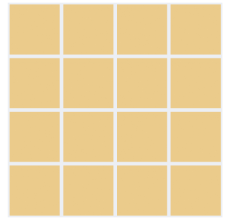
\includegraphics{images/4x4_start_board.PNG}
        \sethebrew
    \end{subfigure}%
    \begin{subfigure}{.5\textwidth}
        \unsethebrew
        \caption{\R{לחיצה על משבצת מסומנת}}
        \centering
        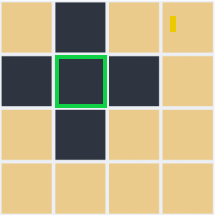
\includegraphics{images/4x4_press.PNG}
        \sethebrew
    \end{subfigure}%
\end{figure}

נבחין כי המשחק 
$4 \times 4$
מתחיל במצב
\L{(a)}.
\\
בלוח 
\L{(b)}
נתאר מצב בו לחצו על משבצת המסומנת, בירוק
כל המשבצות השכנות והיא משנות מצבן, היות ומצב של כולן היה דלוקות לכן הן נכבו

המשחק במקור היה צעצוע אלקטרוני על לוח 
$5 \times 5$
ששוחרר ב 
$1995$.
\\
המשחק יכול להראות פשוט אבל כפי שתואר
במאמר
\cite{B1}
\L{"devilish invention"}.
\\
קיים קושי רב בלמצוא שיטה לפתרון אינטואיטיבי, הקושי של משחק מתבלט בשאלה כיצד כדי להתחיל את המשחק?
\\
בנוסף אציין מניסיון האישי שהמשחק קשה כבר 
על לוח 
$5 \times 5$
ולרוב אנשים שמשחקים אותו מכירים מצבים על הלוח שיודע עליהם משם את הפתרון.

פרויקט זה באה בעקבות הקושי של המשחק
והניסוי להציע שיטות לפתרון, בעקבות ניסיונות עלו
נעזרנו במספר רב של כלים מתמטיים מתקדמים.
\\
אחת המטרות במחקר למצוא הסבר לתופעות במשחק שנתקלנו.

נציין כי קיימים עוד המון שאלות שמשחק מעלה ולא לכולם קיים פתרון,
נשמח בפרויקט זה פתרון לכמה מהשאלות שעולות.
\\
חוץ מאתגר של המשחק עצמו קיים אתגר מתמטי שנרצה בפרויקט זה להציג ולהתעניין.


\subsection{ משחק האורות על גרף}
אחרי שכללי המשחק על לוח הובנו אפשר לנסות להכליל את המשחק כמשחק על גרף.
\\
קיימים הרבה סיבות בהם תירצה להגדיר את הבעיה על מבנה כללי שכזה:

\begin{enumerate}
    \item 
    ככול שמבנה כללי יותר תאוריה שאתה מפתח מתאימה ליותר בעיות.
    \item 
    קיימת תאוריה רחבה שפותחה על גרפים ואתכן שנעזר בחלק
    מהטענות מהתאורה שכזה.
    \item 
    מבליט את מהות הבעיה והגדרה הבסיסית ביותר של המשחק.
\end{enumerate}

ארצה להתייחס לנקודה אחרונה, החשיבות הגדולה שאפשר לתאר את הבעיה של משחק
כאוסף של כללים על גרף, מרכזת אותנו לבעיה ובסופו של דבר כשנראה את שיטה למציאת
הפתרון, השיטה עצמה תזכיר לנו מיד את הייצוג הגרפי.

כדי לתאר את משחק האורות על גרף נשתמש באותם כללים שהגדרנו פרט לעובדה
שצמתים הם הלחצנים או המשבצות במקרה של הלוח
וכל לחיצה הופכת את המצב של הצומת והשכנים שלה.
\\
נזכיר כי צמתים שכנים הם צמתים שיש
קשת ביניהם.

נציין כי כאשר כל צומת יכולה להיות בשתי מצבים,
דלוקה או כבויה המטרה היא לעבור מכל הצמתים במצב מסוים דלוק למצב אחר כבוי.
\\
העובדה שמצב התחלתי הינו דלוק או כבוי אינה תשנה את המשחק עלה רק לאיזה מצב סופי צריך לעבור
לכבוי או דלוק.

נמחיש זאת על דוגמה:
\begin{figure}[ht]
    \begin{subfigure}{.5\textwidth}
        \unsethebrew
        \caption{\R{מצב התחלתי}}
        \centering
        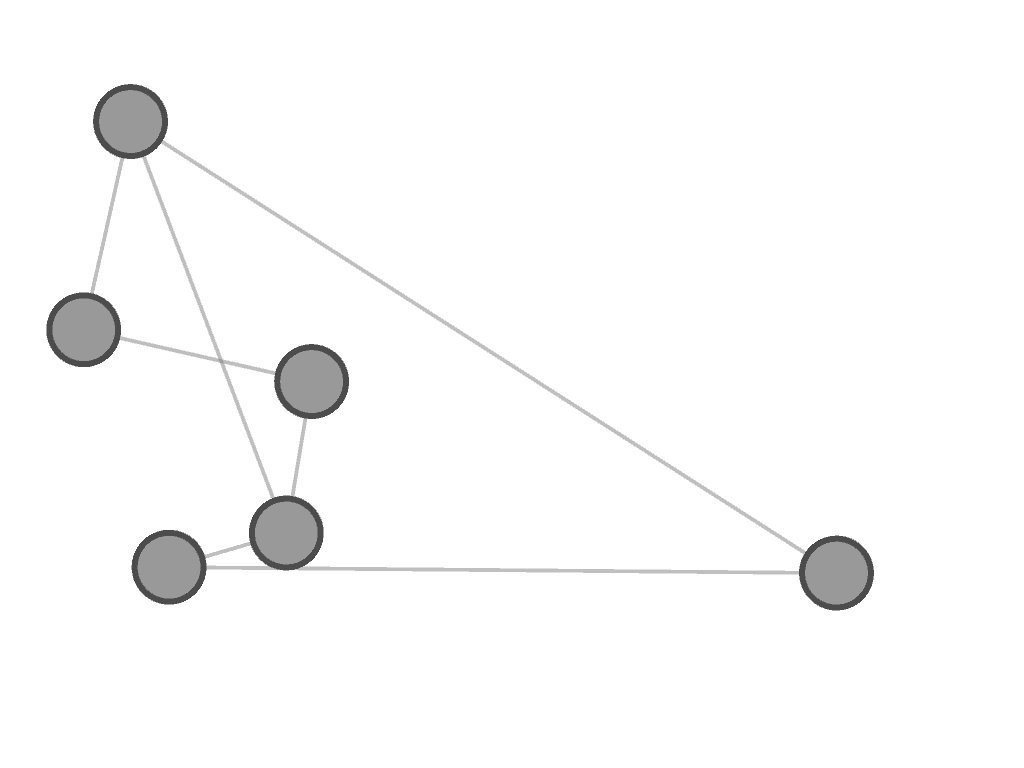
\includegraphics[width=\textwidth,height=\textheight,keepaspectratio]{images/graph_start_board.png}
        \sethebrew
    \end{subfigure}%
    \begin{subfigure}{.5\textwidth}
        \unsethebrew
        \caption{\R{לחיצה על משבצת מסומנת}}
        \centering
        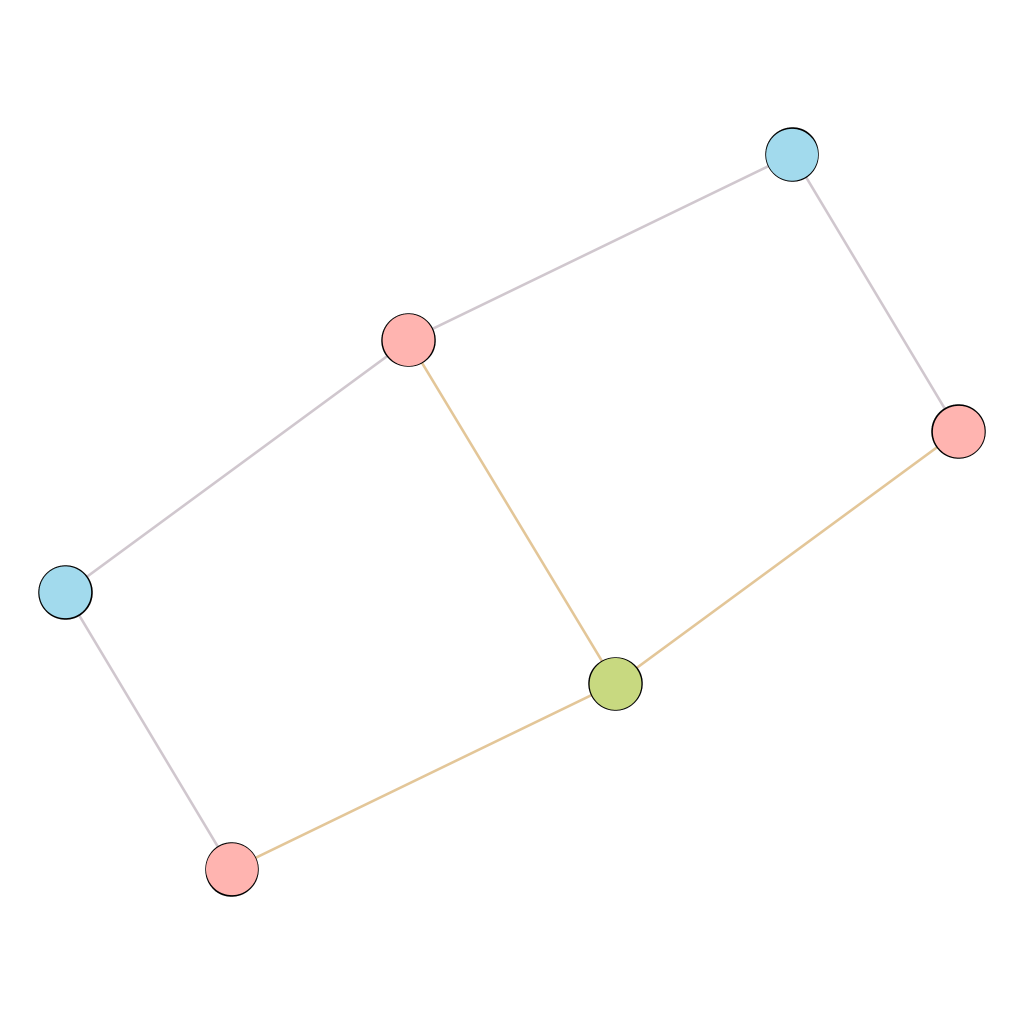
\includegraphics[width=\textwidth,height=\textheight,keepaspectratio]{images/graph_press.png}
        \sethebrew
    \end{subfigure}%
\end{figure}

על גרף התחלתי
\L{(a)}
ניתן לראות
$6$
קודקודיים
צבועים באפור ומטרה לצבוע את כולם לצהוב.
\\
בשלב 
\L{(b)}
מציגים  לחיצה על צומת ירוקה היא ושכניה נצבעים בצהוב.

\begin{comm}
    בפועל צומת ירוקה גם נצבעת לצהוב צביעה לירוק נועדה להדגשה על מי נלחץ
\end{comm}

משחק על גרף הינה הכללה  של משחק על לוח כלומר, כל משחק 
לוח ניתן לתאר בעזרת משחק על גרף.

נמחיש זאת על דוגמה:

ניקח לוח למשל
$2 \times 3$
נמספר את המשבצות כמו באיור
\ref{2x3_board}

\begin{figure}[ht]
    \caption{
        \R{לוח
        $2 \times 3$
        }
    }
    \label{2x3_board}
    \unsethebrew
    \centering
    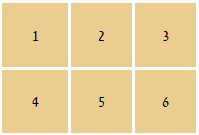
\includegraphics[width=0.5\textwidth,height=0.5\textheight,keepaspectratio]{images/2x3_board.PNG}
    \sethebrew
\end{figure}

כדי לתאר את הלוח על על משחק גרף נשתמש בשני הכללים הבאים:

\begin{enumerate}
    \item 
    כל משבצת על משחק לוח נהפוך לנקודה.
    \item 
    כל זוג משבצות סמוכות על לוח נחבר את נקודות בקו
\end{enumerate}

הגרף שנקבל עבור לוח באיור
\ref{2x3_board}
מתואר באיור
\ref{2x3_graph}

\begin{figure}[ht]
    \caption{
        \R{גרף
        $2 \times 3$
        }
    }
    \unsethebrew
    \centering
    \label{2x3_graph}
    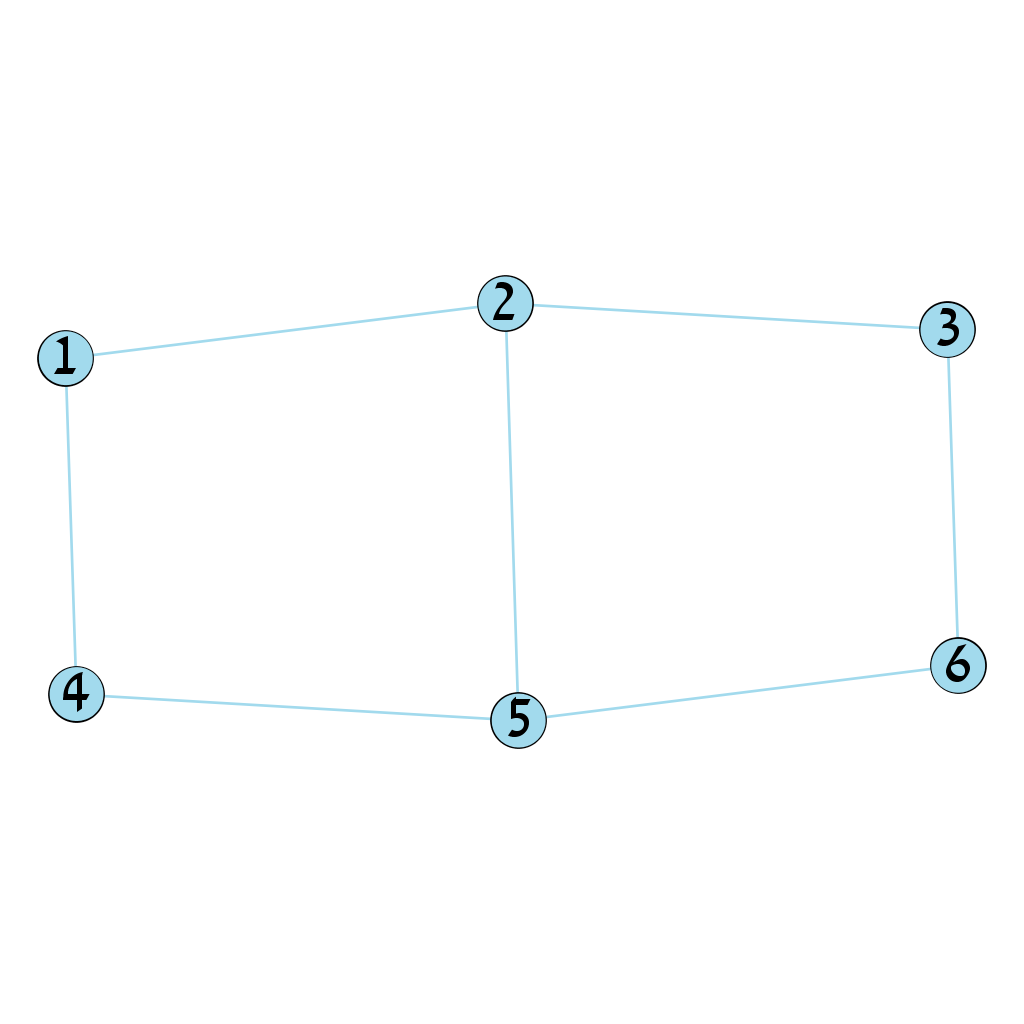
\includegraphics[width=0.5\textwidth,height=0.5\textheight,keepaspectratio]{images/2x3_graph.png}
    \sethebrew
\end{figure}

נשים לב שלגרף בו יש צומת אם יותר מ
$4$
שכנים לא ניתן לתאר לוח שכזה כיוון שלכל היות במשחק על לוח
לכל משבצת יש לכל יותר 
$4$
משבצות סמוכות.

לכן לסיכום אפשר למדל כל משחק לוח על משחק גרף שמייצג אותו אבל 
ההפך זה לא נכון.

\newpage

\section{ אלגוריתם למציאת פתרון}
לפני שנציעה לעלות פתרון, נשאל את עצמנו מדוע בכלל צריך למצוא פתרון.
הרי בסופו של דבר זה משחק ולהציע פתרון למשחק יפגע במהותו משחק הרי אף אחד לא ירצה
לשחק במשהו שידוע מה הפתרון שלו.

הצורך למצוא פתרון הוא נוראה טבעי וזה בעקבות שמששחק עצמו מעניין, כשאתה מתחיל 
את המשחק על לוח 
$3 \times 3$
המשחק ניראה תמים ופשוט אתה מתחיל לצפות לאיזושהי חוקיות.
\\
בשלב הזה שאתה כבר מנסה לוח 
$4 \times 4$
המשחק מתגלה כלא פשוט כשאתה מנסה לוח בקונפיגורציה כלשהי לא בהכרח התחלתית
מהר מאד אתה נעבד.
\\
בשלב מסוים גם לוח 
$4 \times 4$
נהיה מוכר ובאופן תמים תנסה לעבור ללוח
$5 \times 5$
ומהר מאד הלוח שובר את רוחה.
קיימים כל כך הרבה מכירים שנשארת לך משבצת אחת שנותרה לסדר ואינה נעלמת
האינטואיציה שחשבת שפיתח על לוח 
$4 \times 4$
נעלמת כאילו למדת לשחק משחק חדש לגמרי.

התופעה הזאת ששינוי גודל מרגיש שהתחלת משחק אחר עוד
מורגשת בשלב שאתה מנסה לפתור את מצב התחלה בלוחות שונים


\begin{figure}[ht]
    \caption{\R{פתרונות של משחק על לוחות שונים}}
    \unsethebrew
    \label{fig:sol_3_4_5}
    \centering
    \begin{subfigure}[b]{.25\linewidth}
    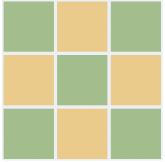
\includegraphics[width=\linewidth]{images/3x3_sol.PNG}
    \end{subfigure}
    \begin{subfigure}[b]{.25\linewidth}
    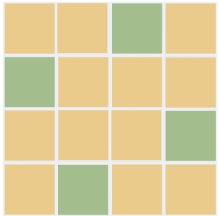
\includegraphics[width=\linewidth]{images/4x4_sol.PNG}
    \end{subfigure}
    \begin{subfigure}[b]{.25\linewidth}
    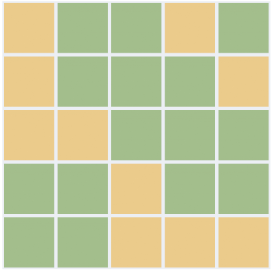
\includegraphics[width=\linewidth]{images/5x5_sol.PNG}
    \end{subfigure}

\end{figure}
\sethebrew

איור
\ref{fig:sol_3_4_5}
באה להמחיש את חוסר  אינטואיציה
כאשר האיור מתאר את פתרון של משחק על הלוח כאשר הלוח במצב התחלתי בו כל נורות דלוקות.
כדי שהשחקן ינצח עליו ללחוץ על המשבצות הירוקות.
\\
איור באה להראות שלוחות על קטנים מ
$5 \times 5$
אתכן ותחשוב שפתרון נוצר על לחיצות סימטריות והאיור ממשיך שזה לא כך 
כי כאשר מסתכלים על הלוח 
$5 \times 5$
מיד אפשר לראות שפתרון לא ניראה סימטרי.

חוסר האינטואיציה מתבלט גם מהעבודה שכמות הפתרונות משתנה לכל לוח.
עבור לוח 
$3 \times 3$
קיים פתרון יחיד,
אבל ללוח 
$4 \times 4$
קיים
$16$
פתרונות.
כמה פתרונות היה ללוח
$5 \times 5$
,
האם זה יותר או פחות מלוח
$4 \times 4$
בהפתעה רבה ללוח 
$5 \times 5$
יש רק 
$4$
פתרונות שזה  מפתיע כי אפשר היה לצפות שמספר פתרונות על לוח גדול יותר אגדל.

אפשר להוסיף שעבור לוחות ריבועים כלומר
$n x n$
כמות הפתרונות כל כך לא צפויה כי עברו 
$n \in [1,20]$
מספר הפתרונות הגדול ביותר הוא ללוח
$19x19$
ומספר פתרונות 
הוא 
$65536$.
מספר הפתרונות השני הגדול ביות הוא רק
$256$.

חוץ מבעיית חוסר אינטואיציה לחיפוש פתרון  טבעי אפשרי לנסות
פתרון נאיבי המנסה כל לחיצה .
\\
פתרון הנאיבי נפסל ברגע הזה שחושבים על כמה קומבינציות לחיצה קיימות.

\begin{lemma}
    כמות האפשרויות לחיצה על לוח
    $m \times n$
    הוא 
    $2^{m \cdot n}$
\end{lemma}
נומר שאפשרויות לחיצה זה חסם על כמות המצבים האפשריים שמשחק יוכל להיות.
חסימה זאת נובעת משאלה אם שחקן לוחץ על לחצן כמה יכול להשפיע על הלוח.
מובן שאם שחקן לחץ על לחצן מספר זוגי של פעמיים המצב יחזור למצב שהיה.
לכן,
כל לחצן משפיע על הלוח אם הוא נלחץ או לא כלומר, יכול להיות בשתי מצבים.
היות וללוח
$m \times n$
קיים 
$m \cdot n$
לחצנים
,
היות וכל לחצן 
יכול להיות בשתי מצבים שונים
לכן נקבל 
שמספר אפשרויות לחיצה 
ללחצן 
$2$
ול
$m x n$
לחצנים
$2^{m \cdot n}$.

כבר בלוח 
$6x6$
כמות  אפשרויות לחיצה גדולה 
מכמות הסטנדרטית שמציגים מספר שלמים,
4 בתים או 
$2^32$
מספרים,
המטרה של המחשה זה להדגיש כמה לא פרקטית אופציית הפתרון שכזה.

עכשיו שיש לנו מוטיבציה למצוא פתרון השאלה היא באיזה כלים בעבודה זה נציע להסתכל על שיטה
הממדל את הבעיה לשדה לינארי ולעזר בכלים של אלגברה לינארית למצוא מספר פתרונות שונים.

% TODO: תאוריה ל שדות סופיים

אתכן ויש כמה דרכים להגיע לאותה מודל לינארי שנציע, נציג בעובדה זה שני דרכים אחת 
בעזרת וקטורי שינוי ומניסיון למצוא צירוף לינארי של וקטורים עלו נמצא את פתרון, דרך שניה תהיה
לפי מערכת משוואות שמתארת את הבעיה.
\\
בשני הדרכים נראה שהגנו לאותה מערכת משוואות ונפתור את המשחק בעזרת חיפוש פתרון של המערכת.
\\
בחרנו להציג קודם בעזרת וקטורי שינוי משום שהגדרת וקטורים פשוטה יותר להסבר לאחר שניראה את הדרך הראשונה
הדרך השנייה קלה יותר להסבר.


כדי למדל את הבעיה על שדה לינארי נזכר בייצוג גרפי שאומר כי לחיצה על צומת משנה את הצומת ושכניה 
אם נסמן את צמתים ב
$n_i$
אז אפשר לתאר כי המצב אתחלתי של משחק על גרף הוא שכל צומת אם הערך התחלתי
$n_i = 0$
וכל צומת יכול לקבל 2 ערכים שנסמן אותם ב
${0,1}$
כאשר 
$0$
מצב התחלתי שכל צמתים התחילו 
ו
$1$
מצב סופי של משחק 
המשחק מסתיים כשכל הצמתים מקיימים
$n_i = 1$.
לכן אנחנו עובדים על שדה בינארי.

אפשר לתאר לחיצה על צומת 
$i$
כווקטור שינוי ערכי צמתי שכנים

לדוגמה ניקח 
משחק בגודל
$2x2$
נמספר את הצמתים 
שורות ואז עמודות מלמעלה למטה כלומר כמו מתואר באיור
\ref{fig:numbering_board_2x2}

\begin{figure}[ht]
    \caption{\R{מספור לוח}}
    \label{fig:numbering_board_2x2}
    \unsethebrew
    \centering
    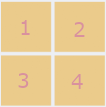
\includegraphics[width=.5\textwidth,height=.5\textheight,keepaspectratio]{images/numbering_board_2x2.PNG}
\end{figure}
\sethebrew

\begin{comm}
    \label{ comm: indexing board game}
    מספור לפי שורה עליונה על כל עמודות עד לשורה תחתונה תהיה שיטת המספור לאורך כל ספר
\end{comm}

לאחר מספור שכזה נוכל לומר שלחיצה על משבצת 
$1$
וקטור שינוי שלה היה
$
    t_1 = 
    \begin{bmatrix}
        1 \\
        1 \\
        0 \\
        1 \\
    \end{bmatrix}
$
\\
$t_1$
מתאר את עלו צמתים יכול שינוי

עבור גרף וקטור שינוי הי כדומה.
\\
עבור גרף באיור 
מתקבל וקטור שינוי של צומת 
$1$
כך
\ref{fig:numbering_graph}
$
    t_1 = 
    \begin{bmatrix}
        1 \\
        0 \\
        1 \\
        1 \\
    \end{bmatrix}
$

\begin{figure}[ht]
    \caption{\R{גרף ממוספר}}
    \label{fig:numbering_graph}
    \unsethebrew
    \centering
    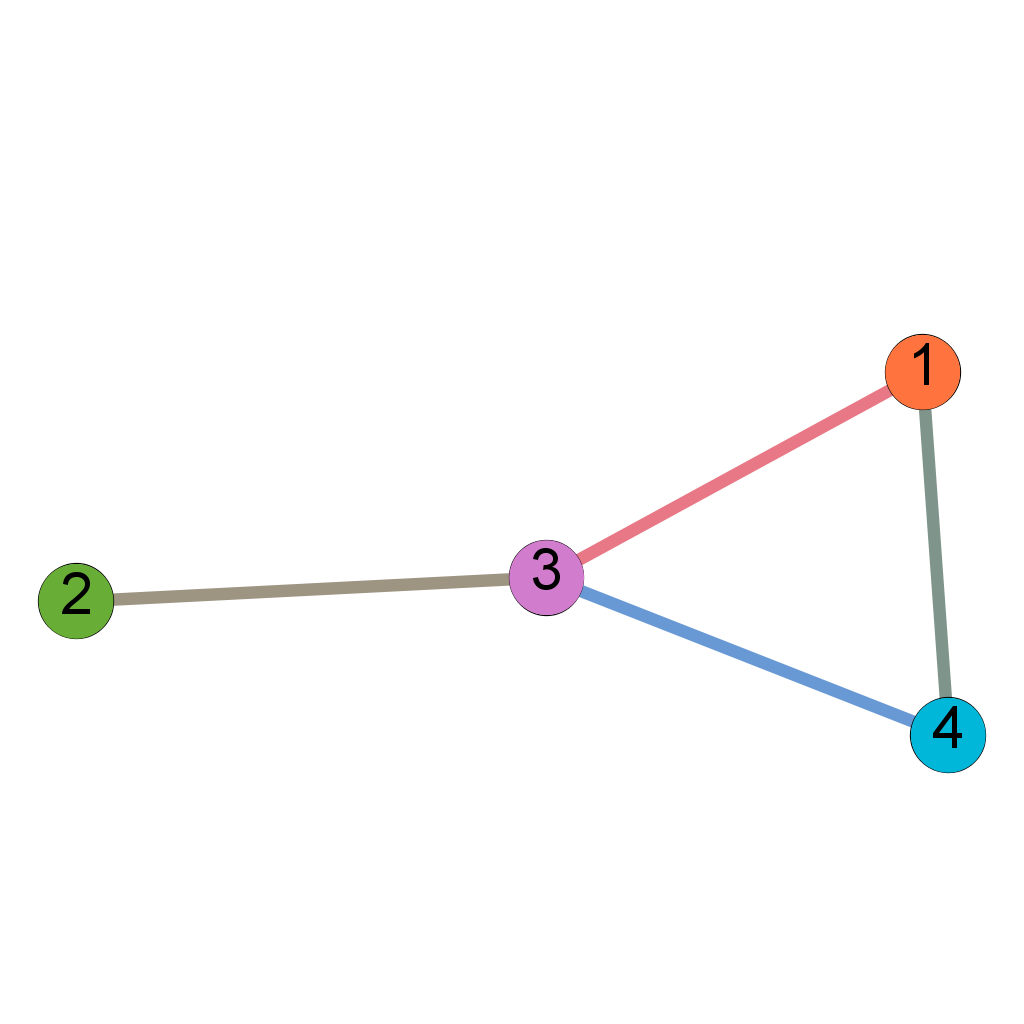
\includegraphics[width=.7\textwidth,height=.7\textheight,keepaspectratio]{images/numbering_graph.PNG}
\end{figure}
\sethebrew

\begin{definition}
    וקטור השינוי
    שנסמן ב
    $\vec{t_j}$
    של לחצן
    ממוספר
    $i$.
    \\
    וקטור
    שייך 
    לשדה 
    $\Zn$
    כאשר 
    $F_2$
    שדה בינארי
    ו 
    $n$
    הינו מספר הלחצנים.
    נגדיר שערכיו
    $t_{i,j} = 1$
    עבור
    לחצנים
    $j$
    שכנים עליו ועל עצמו
    ושאר ערכי וקטור שווים ל
    $0$.
\end{definition}

\begin{comm}
    היות ווקטור שינוי שדה
    $\Zn$
    חיבור בין וקטורים הינו חיבור בין האינדקסים מודול 
    $2$
    וכפל בסקלר
    הוא לכפול את כל ערכי וקטור בסקלר
    כאשר הסקלרים יכולים להיות
    $0$
    או 
    $1$
\end{comm}

נזכיר שלחצנים שכנים הם לחצנים שמשתנים אתו באת לחיצה 
אם זה במקרה הגרפי צמתים שכנים כלומר בעלי צומת משותפת
או במקרה הלוח זה לחצנים בעלי צלע משותפת.

בעזרת וקטורי השינוי אפשר לתאר תוצאה של קומבינציות של לחיצות
בעזרת צירוף לינארי של וקטורי שינויים.
את המצב המתקבל נוסיף למצב הקיים ונקבל את השינוי שנוצר בלחיצה של כפתורים.
נדגים רעיון זה על איור
\ref{fig:start graph presses}
.

נניח שצומת 1 היא יחידה שדלוקה.
\\
נרצה להראות איך הגרף יראה עם ילחצו על כפותרים 
$1, 3$.

\begin{figure}[ht]
    \caption{\R{מצב התחלתי}}
    \label{fig:start graph presses}
    \unsethebrew
    \centering
    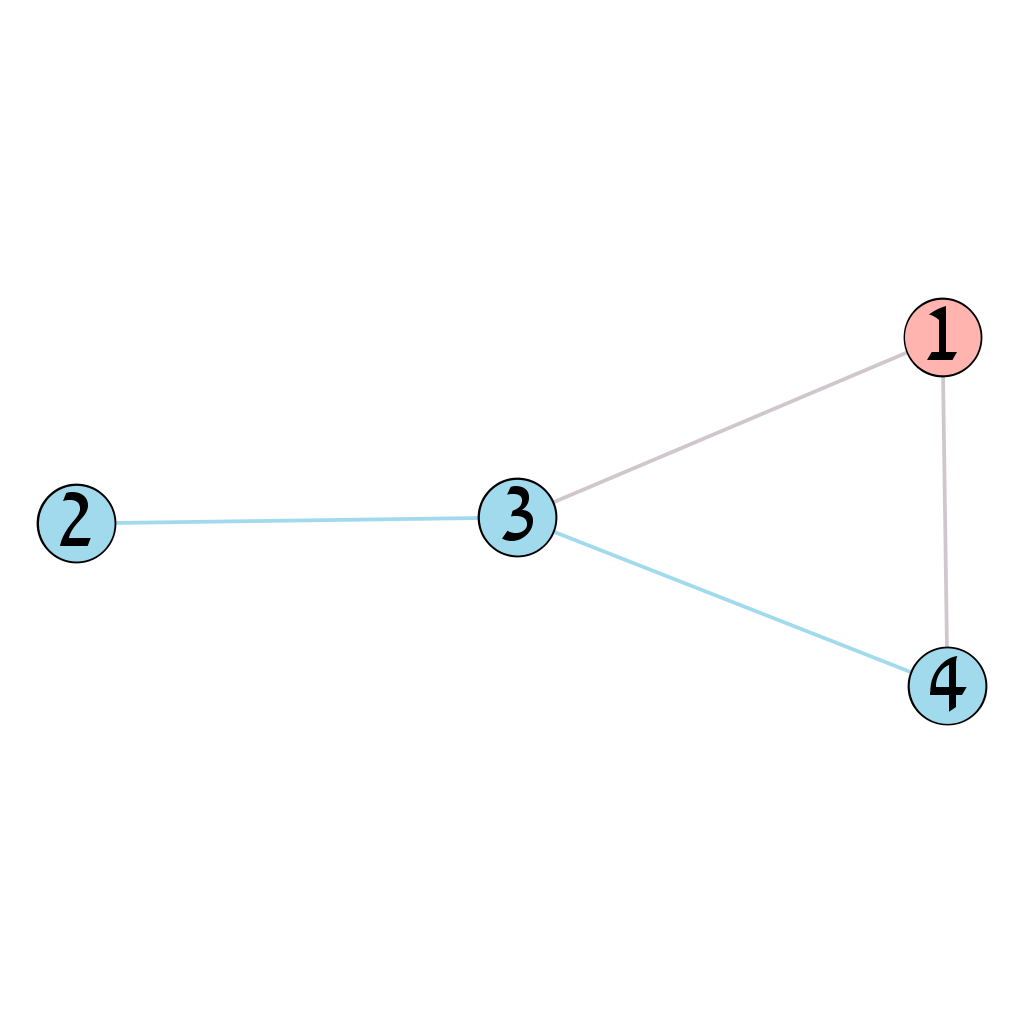
\includegraphics[width=.7\textwidth,height=.7\textheight,keepaspectratio]{images/graph_presses.png}
\end{figure}
\sethebrew

$
    t_1 + t_3 = 
    \begin{bmatrix}
        1 \\
        0 \\
        1 \\
        1 \\
    \end{bmatrix}
    +
    \begin{bmatrix}
        1 \\
        1 \\
        1 \\
        1 \\
    \end{bmatrix}
    =
    \begin{bmatrix}
        0 \\
        1 \\
        0 \\
        0 \\
    \end{bmatrix}
$

ומצב התחלתי שמתואר באיור נסמן ב
$S_0$
לכן מתקבל

$
    S_0 + t_1 + t_3 = 
    \begin{bmatrix}
        1 \\
        0 \\
        0 \\
        0 \\
    \end{bmatrix}
    +
    \begin{bmatrix}
        0 \\
        1 \\
        0 \\
        0 \\
    \end{bmatrix}
    =
    \begin{bmatrix}
        1 \\
        1 \\
        0 \\
        0 \\
    \end{bmatrix}
$

וקטור התוצאה שהתקבל אכן תואם לתוצאה המצופה
מתואר באיור 
\ref{fig:start graph presses solution}.

נשים לב שעבור איך שהגדרנו את המשחק 
\L{Light out}
המשחק מתחיל כשכול
נורות דלוקות או כבויות
ומטרה היא לכבות או להדליק את כל נורות.
\\
כפי שאמרנו שני המשחקים שקולים ההבדל רק
מה המשמעות שנותנים לערכים
$0 ,1 $ 
ומהו מצב הלוח התחלתי בהגדרה זה.

\begin{figure}[ht]
    \caption{\R{מצב לאחר ביצוע הלחיצות}}
    \label{fig:start graph presses solution}
    \unsethebrew
    \centering
    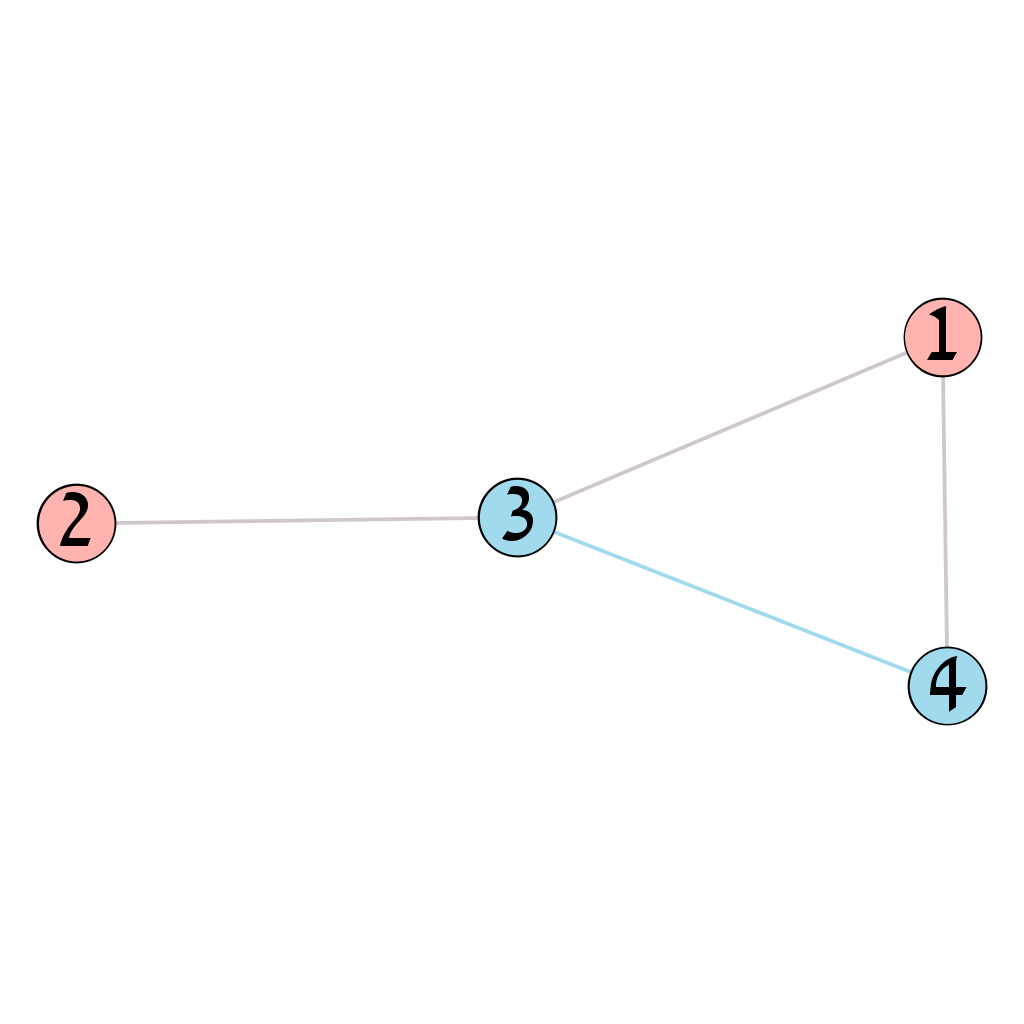
\includegraphics[width=.7\textwidth,height=.7\textheight,keepaspectratio]{images/graph_presses_solve.png}
\end{figure}
\sethebrew

מפרק זה נגדיר שאנחנו פותרים את המשחק שלוח התחלתי כולו באפסים
ומטרה להגיע ללוח שכולו אחדים.
תיאור הטבעי למשחק שכזה להתחיל מלוח כבוי ומטרה להדליק את כל הנורות

מתיאור שכזה מובן כי 
$S_0$
זהו וקטור אפסים לכן כדי לתאר את ממצב התחלתי
למצב לצירוף לינארי של וקטורי שינוי 
אין צורך לחבר בין מצב התחלתי וצירוף לינארי.

היות ומתקיים:

\begin{equation}
    \label{eq: sum change vectors}
    S_0 + \sumi{j} a_i \vec{t_j} =  \sumi{j} a_j \vec{t_j}
\end{equation}

בעקבות כך ניתן לתאר את בעיית המשחק לצורה הבאה:

\begin{equation}
    \label{eq: lin eq for solving problem}
    \sumi{j} a_j \vec{t_j} = \vec{1}
\end{equation}

כאשר
$\vec{1}$
וקטור שכל ערכיו אחדים
ו
$n$
מספר הצמתים בגרף.

תיאור שכזה מדגיש מספר תכונות 

\begin{lemma}
    סדר הלחיצות לא משנה את התוצאה הסופית
\end{lemma}
נשים לב שאם ידוע קבוצת לחיצות ממצב התחלתי הערך של משבצת מסוימת נקבע לפי 
הערך של וקטור תוצאה
בנוסחה
\ref{eq: sum change vectors}.
נשים לב שתוצאת הסכום איננה תלויה בסדר הלחיצות של הוקטור. 

מערכת משוואות 
שמתוארת בנוסחה
\ref{eq: lin eq for solving problem}
אפשר לתאר במספר צורות ונפוצה מבניהם היא
בעזרת מטריצה כמו שמתואר 
בנוסחה 
\ref{eq: matrix eq for solving problem}.

\begin{equation*}
    \begin{bmatrix}
        t_1 & t_2 & \cdots & t_n
    \end{bmatrix}
    \begin{bmatrix}
        a_1 \\
        a_2 \\
        \cdots \\
        a_n \\
    \end{bmatrix}
    =
    \begin{bmatrix}
        1 \\
        1 \\
        1 \\
        1 \\
    \end{bmatrix}
\end{equation*}
\begin{equation}
    \label{eq: matrix eq for solving problem}
    \begin{bmatrix}
        t_{1,1} & t_{1,2} & \cdots & t_{1,n} \\
        t_{2,1} & t_{2,2} & \cdots & t_{2,n} \\
        \cdots & \cdots & \cdots & \cdots\\
        t_{i,j} & t_{i,2} & \cdots & t_{i,n} \\
        \cdots & \cdots & \cdots & \cdots\\
        t_{n,1} & t_{n,2} & \cdots & t_{n,n} \\
    \end{bmatrix}
    \begin{bmatrix}
        x_1 \\
        x_2 \\
        \cdots \\
        x_n \\
    \end{bmatrix}
    = 
    \begin{bmatrix}
        1 \\
        1 \\
        \cdots \\
        1 \\
    \end{bmatrix}
\end{equation}

% TODO: מטריצה שכנות
נבחין שמטריצה בערכים של 
מטריצה במשוואה 
\ref{eq: matrix eq for solving problem}
עבור משחק על גרף.
נשים לב שמטריצה
מטריצה מקבלת ערכים שהם 
$1$
לצמתים שהם שכנים או לעצמם
לכן נגדיר אותה כך.

\begin{definition}
    \label{def: neighbor matrix}
    מטריצה שמתארת את משחק תקראה מטריצת שכנויות של משחק.
\end{definition}


\begin{comm}
    \label{comm: symetic matrix}
    היות וכל צומת שכנה היא שכנה אחד לשני לכן במטריצה
    סימטרית
\end{comm}

המטריצה  המתקבלת מגרף באיור 
\ref{fig:start graph presses solution}:

\[
    \begin{bmatrix}
        1 & 0 & 1 & 1\\
        0 & 0 & 1 & 0\\
        1 & 1 & 1 & 1\\
        1 & 0 & 1 & 1\\
    \end{bmatrix}
\]


\begin{definition}
    \label{ def: solution vector}
    תהי משחק ומערכת משוואת שמתארת אותו מצורה 
    \ref{eq: matrix eq for solving problem} 
    נגדיר את וקטור פתרון כאוסף הלחצנים ומצב להגיע לפתרון
    ונסמן אותו ב
    $\vec{x}$
\end{definition}

הגדרה 
\ref{ def: solution vector}
מתכוונת שאם מתקבל
$\vec{x}$
וקטור פתרון של המערכת 
ו
$x_i = 1$
אז המשמעות שכדי לפתור את המשחק
צריך ללחוץ על לחצן 
$i$.
\\
בנוסף 
$\vec{x}$
אחד הפתרונות אתכן והיו כמה.

\begin{definition}
    \label{def: standard solution}
    שיטת פתרון בעזרת מטריצה תקראה שיטה הסטנדרטית
\end{definition}



תוצאה דומה אפשר לראות בפרק מהספר
\cite{B2}.
\\
מרגע שהצלחנו לתאר את הבעיה מערכת משוואות לינארית
על שדה
$\Zn$
מכן נוכל להיעזר בכלים של אלגברה לינארית כדי למצוא את הפתרון כמו מציאת פתרון בעזרת דירוג,
מציאת מטריצה פסאדו הפוכה וכולי.

\begin{comm}
    \label{comm: for board too many variables}
    עבור לוח 
$[n \times n]$
כמות הלחצנים 
$n^2$
ולכן גודל המטריצה שתוארה במשוואה
\ref{eq: matrix eq for solving problem}
היא 
$[n^2 \times n^2]$
\end{comm}


כלומר כמות הזיכרון שצריך כדי לשמור מטריצה ללוח ריבועי שאורך צלע הוא
$n$
דורש לשמור מטריצה עם 
$n^4$
ערכים
.


\subsection{פתרון בעזרת שיטה הספרדית}
הצגנו גישה פתרון
בגישה הסטנדרטית 
כפי שתיארנו
בהגדרה
\ref{def: standard solution}.
\\
החידה הוצגה כצעצוע ומתאימה למודל שקראנו לו משחק על לוח ריבועי.
לפי הערה 
\ref{comm: for board too many variables}
כמות המידע שצריך לשמור גדל בקצב 
$n^4$
כאשר
$n$
כמות הלחצנים לשורה.
\\
במאמר 
\cite{B1}
מציג שיטה שמציאה פתרון עם מערכת משוואות לינארית אחרת שמובילה גם היא לפתרון.
מערכת משוואת לינארית שמאמר 
\cite{B1}
מתאר ממדי
$n \times n $.
כלומר כמות הערכים המטריצה המתקבלת שווה
ל
$n^2$
שקטנה בריבוע
ממערכת 
שנתונה במשוואה
\ref{eq: matrix eq for solving problem}.

בפרק זה נציג את הגישה שמתוארת 
\cite{B1}
נתאר כמה הבחנות שיסתמכו ששני הגישות שקולות ושגישה החדשה הינה רק אופטימיזציה
ספציפית לצורה של מטריצה הנתונה.
את הגישה החדשה ניקרא לאורך כל הפרק הגישה הספרדית.

\begin{definition}
    \label{def: spanish way}
    גישה הספרדית גישה פיתרון שניה שנציג בעבודה זה.
\end{definition}

נתאר את הגישה הספרדית 
זה הינה גישה שמתאימה לכל גודל של לוח משחק.
כדי להקל על תיאור 
בעזרת דוגמה על לוח 
$3 \times 3$

נניח שאיור 
\ref{fig: 3 x 3 board indexed}
מתאר את הלוח הנתון כאשר המשבצות הינן הלחצנים ומספור זה אינדקסים הערה 
\ref{ comm: indexing board game}
כאשר מתחילים את המספור מ
$0$
נפוץ בשפות תוכנה להתחיל מאינדקס 
$0$.

\begin{figure}[ht]
    \caption{לוח 
    $3 \times 3$
    עם אינדקסים}
    \label{fig: 3 x 3 board indexed}
    \unsethebrew
    \centering
    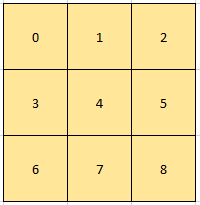
\includegraphics[width=.3\textwidth,height=.3\textheight,keepaspectratio]{images/3x3_board_index.PNG}
\end{figure}
\sethebrew

שיטת הפתרון של מאמר הספרדי הינה להתחל את הלוח עם משתנים ולמלאות את הלוח במשתנים עלו.
לאחר שכל הלוח מלא מתקבלים 
$n$
משוואות במקרה של דוגמה 
$3$
וכל משוואה תהיה עם 
$n$
נעלמים
ולכן נקבל מערכת משוואת שמטריצה המייצגת הינה מסדר 
$n \times n$

שיטת הספרדית מתחיל בכך
שממלאים את השורה העליונה במשתנים
כפי שמתואר באיור 
\ref{fig: 3 x 3 board init spanish}.
לאחר מכן עוברים שורה שורה 
וממלאים אותה במשתנים שמשפיעים על הלחצן.

בשלב זה נסביר את אופן המילוי ומשמעות המשתנים.

ונסמן ב
$x_i$
אם נילחץ על לחצן 
$i$.
אם נתייחס לכל הלחצנים כווקטור מסודר לפי אינדקס
$i$
נקבל 
$\vec{x}$
כפי שהגדרנו בהגדרה 
\ref{ def: solution vector}.

נתסכל על איור 
\ref{fig: 3 x 3 board indexed}
היות ומטרה להפוך את מצב הלחצנים
כלומר צריך שכמות לחיצות על לחצנים שמשפיעים על 
משבצת סכום במודול
$2$
היה 
$1$
כי 
הלחצן אשאר דלוק.

נדגים
על כמה לחצנים מאיור  
\ref{fig: 3 x 3 board indexed}.
מצב הלחצן תלוי האם הלחצנים 
סמוכים לו  ועצמו לחוצים .
\\
עבור 
לחצן 
$0$.
מתקבלת המשוואה:

\[ x_0 + x_1 + x_3 = 1\]

ועבור לחצן 
$3$:

\[ x_0 + x_3 + x_4 + x_6 = 1 \]

וכך ניתן להגדיר אילוצים לכל הלחצנים.

\begin{definition}
    \label{ def: depndeciy equation}
    המשוואה המתקבלת
    עבור לחצן 
    $i$
    מחיבור מודל 
    $2$
    עם לחצות על הלחצנים המשפעים על לחצן 
    תקראה
    משוואת אילוץ על לחצן 
    $i$
\end{definition}

עבור משחק לוח
ריבועי באורך שורה 
$n$
שהלחצנים ממספרים לפי הערה
\ref{ comm: indexing board game}
ניתן לנסח בנוסחה פשוטה:
\begin{equation}
    \label{eq: depndeciy equation}
    x^*_{i - n} + x^*_{i - 1} + x^*_{i} + x^*_{i + 1} + x^*_{i + n} = 1
    \hspace{10pt}
    x^*_i =
    \begin{cases}
        x_i & \text{if $i \in [1,n^2]$} \\
        0 & \text{otherwise}
    \end{cases}
\end{equation}

\begin{figure}[ht]
    \caption{לוח 
    $3 \times 3$
    מאותחל}
    \label{fig: 3 x 3 board init spanish}
    \unsethebrew
    \centering
    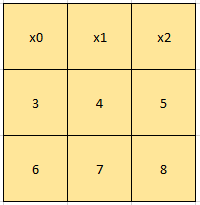
\includegraphics[width=.3\textwidth,height=.3\textheight,keepaspectratio]{images/3x3_first_row.PNG}
\end{figure}
\sethebrew

לאחר שהגדרנו את משוואת האילוצים נסביר כיצד למלאה 
את השורות לפי השיטה הספרדית.
\\
כל לחצן ימלא לפי משוואת האילוצים של הלחצן שמעליו.
\\
כלומר 
כדי למלאה את לחצן 
$3$
נסתכל על משוואת האילוצים של לחצן 
$0$.

\[ x_0 + x_1 + x_3 = 1\]

ניזכר כי המשוואה שהתקבלה הינה על שדה מודול
$2$.
לכן בעזרת העברת אגפים מתקבל.

\[ x_3 = 1 + x_0 + x_1 \]

ונכתוב ערך זה בלחצן 
$3$
כמו שמתואר באיור 
\ref{fig: 3 x 3 board fill button 3}

\begin{figure}[ht]
    \caption{לוח 
    $3 \times 3$
    מילוי משבצת
    $3$}
    \label{fig: 3 x 3 board fill button 3}
    \unsethebrew
    \centering
    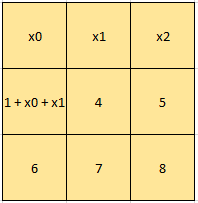
\includegraphics[width=.3\textwidth,height=.3\textheight,keepaspectratio]{images/3x3_fill_button_3.PNG}
\end{figure}
\sethebrew

נשים לב שבעזרת גישה שתיארנו כרגע נוכל למלאה כל השורה שניה.
כל שורה תלויה בשורה מלפניך לכן כך נוכל למלאה את כל השורות 
כמו שמתואר באיור 
\ref{fig: 3 x 3 board fill intire board}

נדגים מילוי משבצת
$6$
משורה שלישית לכן נצטרך ששורה
שניה חושבה.
\\
נסתכל על משבצת מעל 
כלומר משבצת 
$3$
ונסתכל למה שווה משוואת האילוצים שלה:

\[ x_0 + x_3 + x_4 + x_6 = 1 \]

לכן 

\[ x_6 = 1 + x_0 + x_3 + x_4  \]

היות ושורה שניה מולאה וידוע שערך משבצות 
באותה שורה: 

\begin{align*}
    x_3 &= 1 + x_0 + x_1 \\
    x_4 &= 1 + x_0 + x_1 + x_2
\end{align*}
    


נציב ערכים אילו

\begin{align*}
    x_6 &= 1 + x_0 + (1 + x_0 + x_1) + (1 + x_0 + x_1 + x_2) \\
    x_6 &= 1 + x_0 + x_2
\end{align*}

\begin{figure}[ht]
    \caption{לוח 
    $3 \times 3$
    מלאה}
    \label{fig: 3 x 3 board fill intire board}
    \unsethebrew
    \centering
    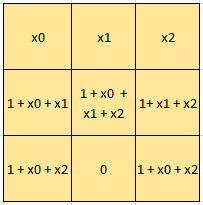
\includegraphics[width=.3\textwidth,height=.3\textheight,keepaspectratio]{images/3x3_fill_all.PNG}
\end{figure}
\sethebrew

כדומה נעשה לשאר הערכים.
התוצאה מתקבלת מתוארת באיור 
\ref{fig: 3 x 3 board fill intire board}

נבחין שלאחר שמילאנו את כל הלוח כמו שמתואר באיור 
\ref{fig: 3 x 3 board fill intire board}
נותרו לנו עוד 
$n$
משוואות אילוץ שתלויות בשורה אחרונה ולכן מאמר 
\cite{B1}
מציאה להוסיף שורה וירטואלית כדי להשתמש 
במשוואות עלו
כמו שמתואר באיור 
\ref{fig: 3 x 3 board fill with virtual}

\begin{figure}[ht]
    \caption{לוח 
    $3 \times 3$
    מלאה
    כולל שורה וירטואלית
    }
    \label{fig: 3 x 3 board fill with virtual}
    \unsethebrew
    \centering
    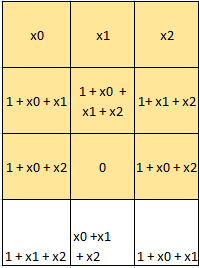
\includegraphics[width=.3\textwidth,height=.3\textheight,keepaspectratio]{images/3x3_fill_virtual.PNG}
\end{figure}
\sethebrew

המאמר טוען שהיות שורה זה לא באמת קיימת לכן
ערכי 
של משבצת המתקבלות 
חייב להיות שווה 
ל
$0$

ולכן קיבלנו 
$n$
משוואת על 
$n$
נעלמים 
כאשר בדוגמה שלנו 
$n=3$
לכן אפשר לנסות לפתור את המערכת הנתונה.

שיטה תוארה על מעבר על שורות אפשר היה לעשות בניה דומה גם לעמודות.

המאמר 
\cite{B1}
מתאר מספר רב של פתרונות  בלוחות ריבועים בגדלים שונה ואפילו על לוחות מלבניים.
\\
האתגר המרכזי בשיטה הספרדית היא להצדיק אותה למה יש שורה וירטואלית
והאם יש קשר בין שני השיטות.
\\
בשלב זה נתרכז להראות את הקשר בין שיטה הספרדית ושיטה שהצגנו בפרק הקודם.

\begin{theorem}
    משוואות האילוצים מתארות את מערכת המשוואות 
    \ref{eq: matrix eq for solving problem}.
\end{theorem}
משוואות האילוצים פורמלית היא לב השיטה הספרדית
מכיוון שהתקדמות בשורות מבוססת על המשוואות עלו.

אם נפרוס את משוואת האילוצים נקבל גם מערכת משוואת שפותרת את המשחק
אבל כמות המשואות הינה 
$n^2$.
נבחין שאם נציג אותם כמטריצה נקבל את מטריצה במשוואה 
\ref{eq: matrix eq for solving problem}
וזאת מכיוון 
שאם נמספר ב
$j$
את כל המשוואות לפי 
האינדקס
$i$.
\\
מתקבל משוואת האילוצים שמשתנה 
$x_i$
מופיעה בהם
באותם אינדקסים 
$j$
שבהם 
וקטור השינוי של לחצן
$i$
מקבל ערכים 
שווים
ל
$1$.


נדגים זאת על לוח 
$2 \times 2$
שמתואר באיור 

\begin{figure}[ht]
    \caption{לוח 
    $3 \times 3$
    מלאה
    כולל שורה וירטואלית
    }
    \label{fig: 2 x 2 board}
    \unsethebrew
    \centering
    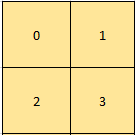
\includegraphics[width=.3\textwidth,height=.3\textheight,keepaspectratio]{images/2x2_board.PNG}
\end{figure}
\sethebrew

וקטורי השינויים:

\[
   t_0 = 
    \begin{bmatrix}
        1 \\
        1 \\
        1 \\
        0 \\
    \end{bmatrix},
    t_1 = 
    \begin{bmatrix}
        1 \\
        1 \\
        0 \\
        1 \\
    \end{bmatrix},
    t_2 = 
    \begin{bmatrix}
        1 \\
        0 \\
        1 \\
        1 \\
    \end{bmatrix},
    t_3 = 
    \begin{bmatrix}
        0 \\
        1 \\
        1 \\
        1 \\
    \end{bmatrix},
\]
לכן
המטריצה מהצורה:
\[
    \begin{bmatrix}
        1 & 1 & 1 &0 \\
        1 & 1 & 0 & 1 \\
        1 & 0 & 1 & 1 \\
        0 & 1 & 1 & 1 \\
    \end{bmatrix},
\]

ומשוואת האילוצים
מהצורה 

\begin{align*}
    x_0 + x_1 + x_2 &= 1\\
    x_0 + x_1 + x_3 &= 1\\
    x_0 + x_2 + x_3 &= 1\\
    x_1 + x_2 + x_3 &= 1
\end{align*}

תעלומה נוספת בשיטה הספרדית היא למה צריך שורה וירטואלי, למה ערכה 
שווה ל
$0$
ואיך המערכת משוואת שלו מצטמצמת ל
$n$
משתנים
\\
הסבר לתופעה זה
ניתן בעזרת הצגה המטריצה
נראה זאת על מטריצה 
של משחק 
על לוח 
$3 \times 3$

נשים לב ששיטה הספרדית מדרג את המטריצה מורחבת 
$[M | \vec{1}]$.

\begin{center}
    \begin{tabular}{|ccccccccc|c|}
        \hline
        1& 1& 0& 1& 0& 0& 0& 0& 0& 1 \\
        1& 1& 1& 0& 1& 0& 0& 0& 0& 1 \\
        0& 1& 1& 0& 0& 1& 0& 0& 0& 1 \\
        1& 0& 0& 1& 1& 0& 1& 0& 0& 1 \\
        0& 1& 0& 1& 1& 1& 0& 1& 0& 1 \\
        0& 0& 1& 0& 1& 1& 0& 0& 1& 1 \\
        0& 0& 0& 1& 0& 0& 1& 1& 0& 1 \\
        0& 0& 0& 0& 1& 0& 1& 1& 1& 1 \\
        0& 0& 0& 0& 0& 1& 0& 1& 1& 1 \\
        \hline
    \end{tabular}
\end{center}

נבחין כי מילוי משבצת 
בשיטה הספרדית היא שקולה להצבה 
שורה קודמת.
פעולה דומה להצבה היא 
דירוג שורה 
לפי משתנה זה.
\\
כלומר מתקבל שזה אותה ששיטה הספרדית הינה 
שיטה חכמה לדרג את הבעיה
עד שנותר 
$n$
משוואות.

המטריצה המדורגת המתקבלת
מלוח 
$3 \times 3$
   

\begin{center}
    \begin{tabular}{|ccccccccc|c|}
        \hline
1& 1& 0& 1& 0& 0& 0& 0& 0& 1 \\
1& 1& 1& 0& 1& 0& 0& 0& 0& 1 \\
0& 1& 1& 0& 0& 1& 0& 0& 0& 1 \\
1& 0& 1& 0& 0& 0& 1& 0& 0& 1\\
0& 0& 0& 0& 0& 0& 0& 1& 0& 0\\
1& 0& 1& 0& 0& 0& 0& 0& 1& 1\\
0& 1& 1& 0& 0& 0& 0& 0& 0& 1\\
1& 1& 1& 0& 0& 0& 0& 0& 0& 0\\
1& 1& 0& 0& 0& 0& 0& 0& 0& 1\\
        \hline
    \end{tabular}
\end{center}

נבחין שמשבצת שחושבו
שהם משבצות 
מ
$3$
עד 
$8$
באיור
\ref{fig: 3 x 3 board indexed}
בשיטה הספרדית
שקולה לשורה 
$i-3$
במטריצה המורחבת המדורגת.

לסיכום השיטה הספרדית היא שקולה לדירוג חכם של המטריצה.
אפשר לומר שמספיק היה לדרג רק 
$n$
שורות אחרונות ומטריצה תהיה מדורגת 
אין צורך את כל השלבים.

לפי חישוב סיבוכיות
לדרג מטריצה 
בגודל 
$n^2 \times n^2$
זה 
$O(n^4)$
דירוג בעזרת שיטה הספרדית אומרת
שעל כל עמודה 
וקטור שינויים 
יש לכל יותר
$5$
ערכים ששווים 
$1$.
לכן הסיבוכיות 
$O(n^2)$
.
\\
אם נעבוד בשיטה 
שרק צריך לדרג את
$n$
שורות 
אחרונות
הסיבוכיות 
$O(n^3)$.

ננסה להראות זאת בפועל על ידי חישוב זמני חישוב.

\begin{figure}[ht]
    \caption{ 
    גרף מתאר ביצועים על לוח ריבועי גודל שורה מול זמן
    }
    \label{fig:prefofmance_diagram}
    \unsethebrew
    \centering
    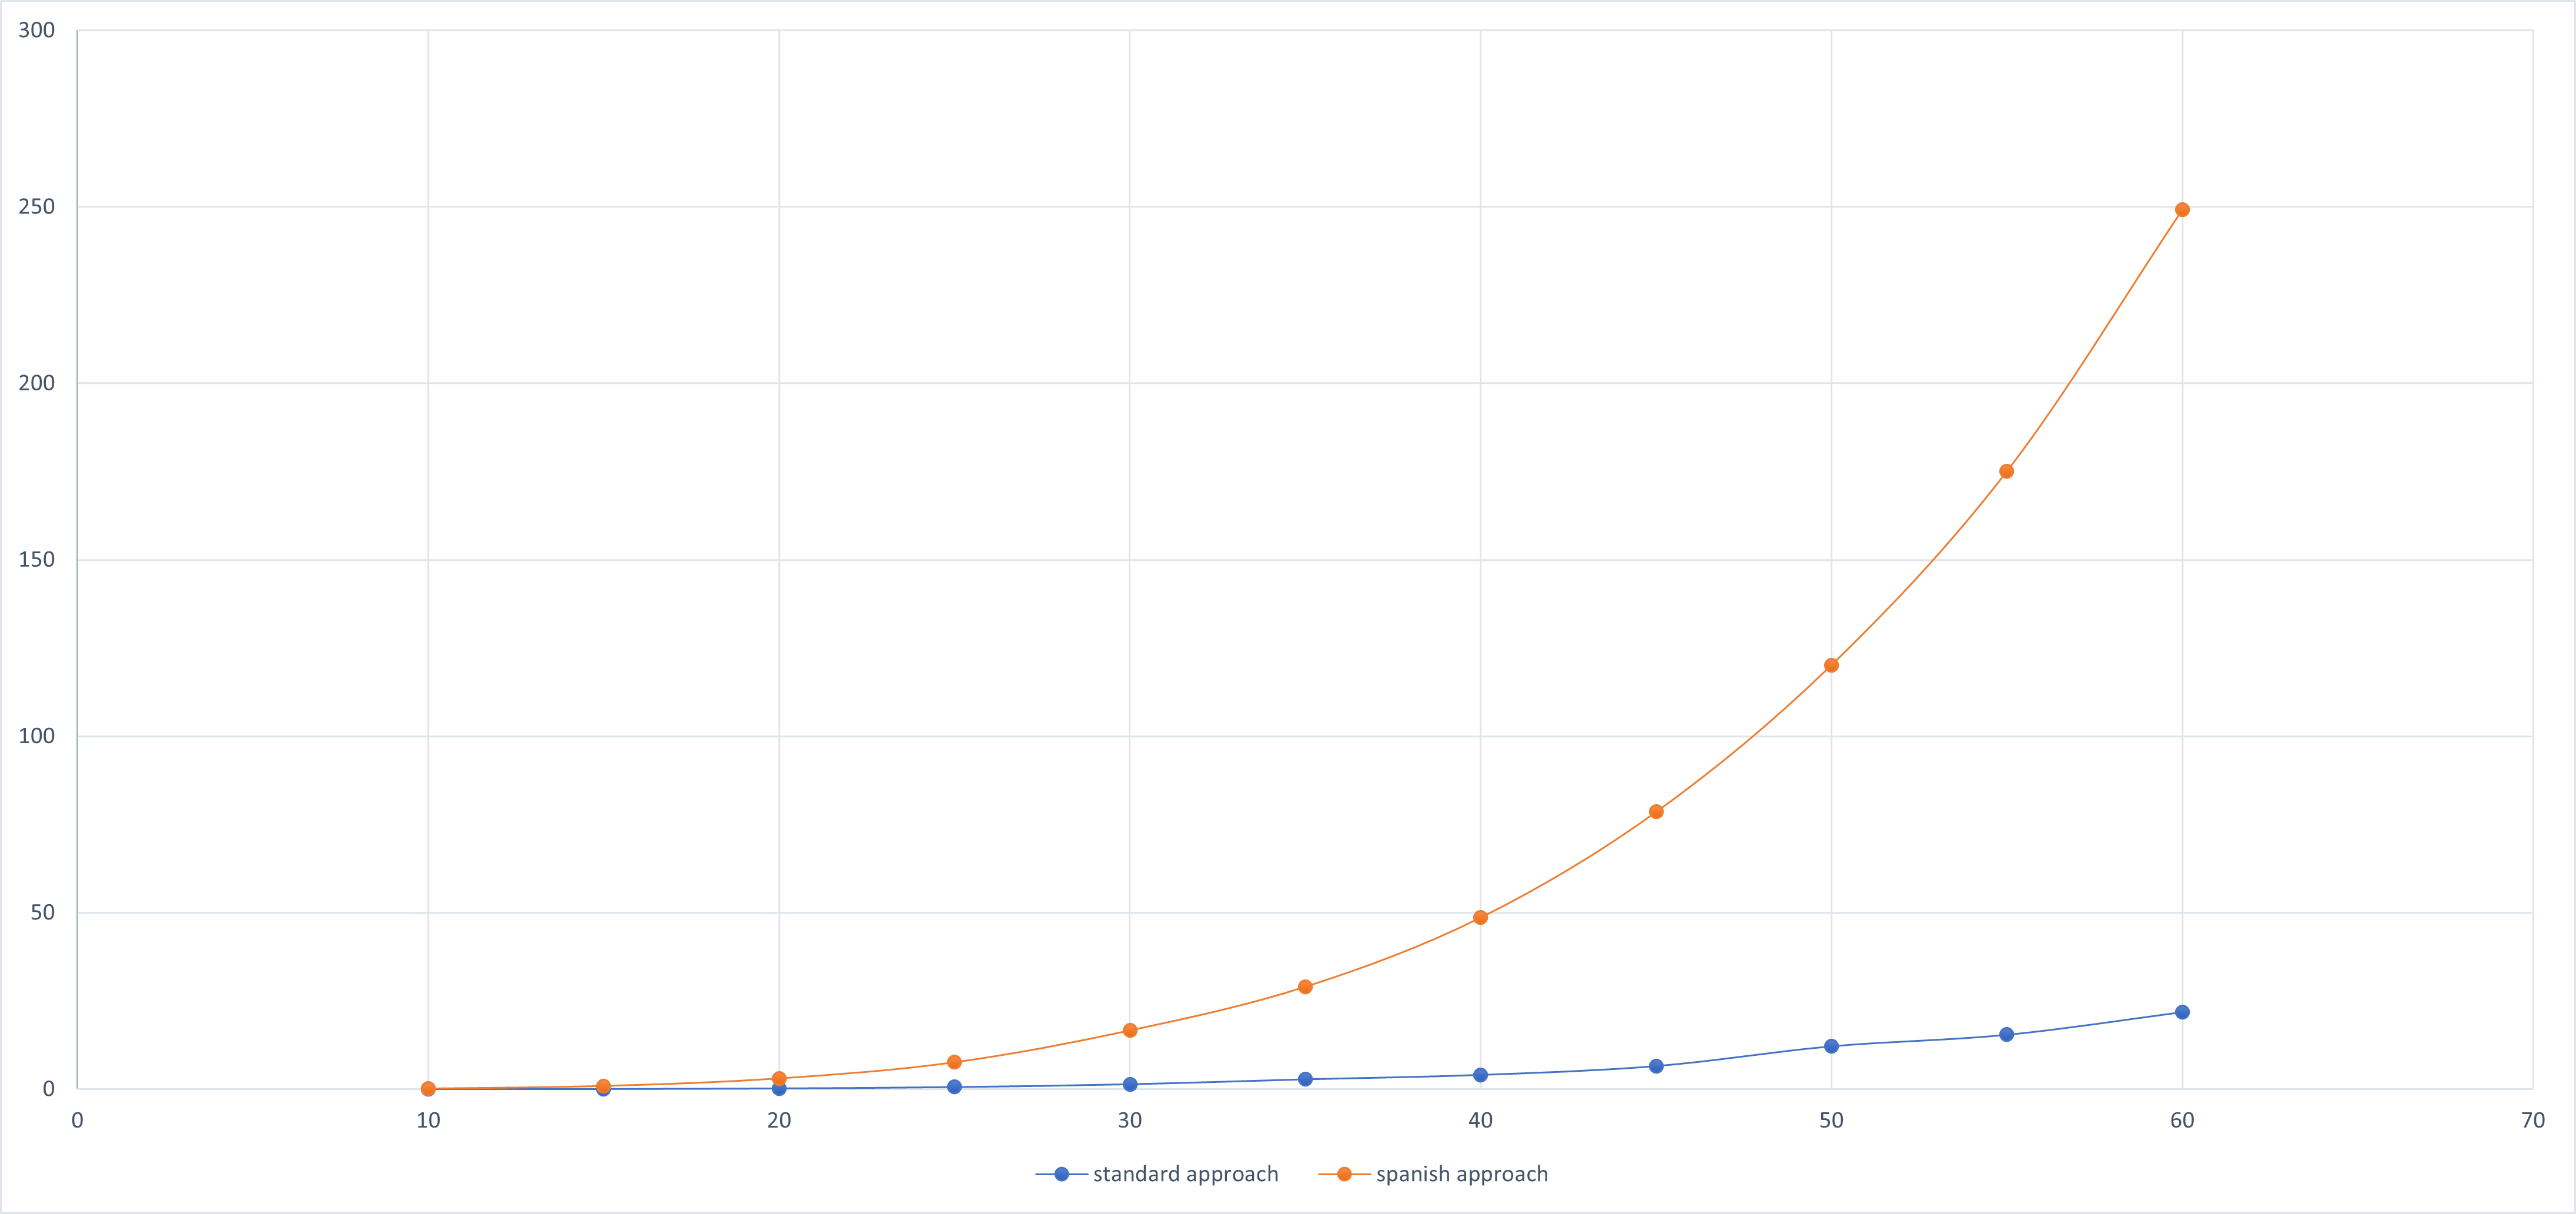
\includegraphics[width=\textwidth,height=\textheight,keepaspectratio]{images/benchmark.png}
\end{figure}
\sethebrew

באיור 
\ref{fig:prefofmance_diagram}
אפשר לראות ביצועים
של שני האלגוריתמים ציר 
ה
$x$
גודל שורה של לוח המלבני
הרצנו על 
לוח בגדלים 
מ
$10$
עד 
$60$
משבצות.
ציר ה
$y$
זמן שלקח 
בשניות
\\
לפי התוצאות של איור 
\ref{fig:prefofmance_diagram}
ניראה 
שגישה הספרדית שבתאוריה יותר אופטימליות לוקחת יותר זמן.
אחת הסיבות לקח היא שאלגוריתם שפותר את מערכת המשוואת אינו עובד בשיטת הדירוג
הוא פונקצית ספריה שמימוש אופטימלי וכניראה מומש לפתור את המערכת בחישוב מקבילי.
לכן ניסיונות להקטין  את המטריצה לא תורם מספיק ליעילות.

\newpage
\section{הוכחת  קיום פתרון עבור כל גרף}
עד כה היסכלנו על שני גישות שונות למציאת פתרון
אבל שאלה טבעית לשאול היא האם בכלל קיים פתרון למשחק על לוח כלשהו?
אחת הדרכים לענות על שאלה שכזה היא פשוט לקחת את הלוח ולפתור בעזרת 
דרכי הפתרון שהצגנו.
אחת הבעיות בגישה של לחפש פיתרון על לוח היא חישובית אני ארצה 
לבדוק על מספר רב של לוחות אם הם פתירים אצתרך להרציץ
את האלגוריתם לחיפוש פיתרון אותו מספר פעמים
לכן, נרצה בשיטה מתמטית להוכיח לעבור איזה משחקים יש פיתרון.
בנוסף חוץ מזה שהלוח שבדקנו פתיר שאלה אחרת היא לבדוק כמה פיתרונות יש ללוח.
מספר הפיתרונות של הלוח יכול להעיד האם הלוח יותר קל או קשה לשחקן שמנסה לפתור אותו
לבד ללא אלגוריתם.
וזה במה שנעסוק בפרק זה.

אחד המקומות ששאלה זה נשאלה היא בספר 
\cite{B3},
בעבודתנו נראה הוכחה קצת שונה בעזרת הכלים שפיתחנו.

\begin{definition}
    \label{def:inner_mul}
    נגדיר פעלוה 
    בין שני וקטורים ב
    $\Zn$
    ניקרא לה מכפלה סקלארית
    תסומן 
    $x \cdot y$
    ונגדיר אותה כך:
    \\
    תהי 
    $\vec{x}, \vec{y} \in \Zn$
    אז 
    \[
        \vec{x} \cdot \vec{y} = 
        \begin{bmatrix}
            x_1 \\
            x_2 \\
            \cdots \\
            x_n \\
        \end{bmatrix}
        \cdot 
        \begin{bmatrix}
            y_1 \\
            y_2 \\
            \cdots \\
            y_n \\
        \end{bmatrix}
        = 
        x_1 y_1 + x_2 y_2 + \cdots x_n y_n
    \]
    כאשר 
    פעולת חיבור בין האיברים 
    הינה 
    חיבור מודול
    $2$
\end{definition}

\begin{comm}
    \label{comm:not_really_inner_mul}
    המכפלה הסקלרית שהגדרנו ב
    \ref{def:inner_mul}
    אינה מכפלה פנימית היות ותכונה 
    $<\vec{u},\vec{u}> = 0 \Leftrightarrow \vec{u} = \vec{0} $
    לא מתקיימת.
\end{comm}

דוגמה 
להסברה הערה
\ref{comm:not_really_inner_mul}:

\[
    \begin{bmatrix}
    1 \\
    1 \\
    \end{bmatrix}    
    \cdot 
    \begin{bmatrix}
    1 \\
    1 \\
    \end{bmatrix} 
    = 1 + 1 = 0
\]

\begin{comm}
    וקטורים 
    $\vec{x}. \vec{y} \in \Zn $
    יקראו מאונכים אחד לשני נסמן זאת 
    $\vec{x} \perp  \vec{y}$
    אם המכפלה הסקלארית שהלם שווה 
    ל
    $0$
    $\vec{x} \cdot \vec{y} = 0$
\end{comm}

\begin{theorem}
    \label{the: Nul A and Col AT}
    תהי מטריצה 
    $A \in {Z_2}^{m \times n }$
    אז 
    $ColA^T \perp Nul A$
    $ColA \perp Nul A^T$
\end{theorem}

ידוע שתכונה זה מתקיימת 
ב
מטריצה 
$A \in R^{m \times n}$
ההוכח 
ל
$ {Z_2}^{m \times n}$
זה
פרט ל
למכפלה הפנימית 
שדורשת 
לבצע על תוצר 
ב
$R^{m \times n}$
עוד 
מודל 
$2$.
היות ותוצר של מכפלה פנימית הינו אפס 
אשראר גם לאחר מודל 
$2$
היה 
$0$.


\begin{theorem}
    \label{thrm: clean game has solution}
    לכל משחק על גרף כאשר המצב התחלתי בו כל הנורות כבויות קיים פיתרון למשחק.
\end{theorem}
לפי 
שיטת פיתרון סטנדרטית 
שהגדרנו
\ref{def: standard solution}
ניתן לתאר את פיתרון המשחק על גרף בעזרת מטריצה
שכנויות לפי הגדרה 
\ref{def: neighbor matrix}.
מטריצה שכנויות
נסמן אותה ב
$A \in {Z_2}^{n \times n}$.
\\
נזכיר כמה תכונות חשובות
\begin{enumerate}
    \item 
    מטריצה סימטרית לפי
    \ref{comm: symetic matrix}
    \item 
    $A$
    המטריצה הינה ריבועית.
    \item 
    האיברים על האלכסון
    מטריצה 
    $A$
    ערכם שווה ל
    $1$.
\end{enumerate}

כדי להראות שלמשחק יש פתרון 
צריך להראות שקיי פתרון למערכת 
\[A \vec{x} = \vec{1} \]

במקרה ש 
$A$
מטריצה הפיכה אז קיים פתרון יחיד.
עבור המקרה שמטריצה אינה הפיכה 
כלומר 
$Nul A \neq \{ \vec{0}\}$
ניקח 
$\vec{x} \in Nul A$
כלומר 
$A\vec{x} = \vec{0} \\$
$\vec{x}^T A \vec{x} = \vec{x}^T\vec{0} = 0 \\$
נסמן 
$\vec{x} = [x_1, x_2, \cdots, x_n]^T$

\begin{multline}
    \label{eq: quadratic form}
        \vec{x}^T A \vec{x} = a_{1,1}x_1^2 + 2(a_{1,2} + a_{2,1})x_1x_2 + \cdots 2(a_{1,n} + a_{n,1})x_1x_n + \\
        + a_{2,2}x_2^2 +  2(a_{2,3} + a_{3,2})x_2x_3 + \cdots  + 2(a_{2,n} + a_{n,2})x_2x_n + \cdots
\end{multline}

היות ומטריצה סימטריות
$a_{i,j} = a_{j,i}$
לכן
מתקבל
\[a_{i,j} - a_{j,i} = a_{i,j} + \cdots + a_{j,i} = 1 \]
נזכיר כי תוצאות של פעולת חיבור וחיסור מודל 
$2$
זהות.

לכן
את המשוואה 
\ref{eq: quadratic form}
אפשר לפשט ל
\[ \vec{x}^T A \vec{x} = a_{1,1}x_1^2 + a_{2,2} x_2^2 +  a_{n,n} x_n^2\]

הבחנה נוספת לערך 
$0$
או
$1$
$x^2 = x$
לכן פישוט נוסף למשוואה 
\ref{eq: quadratic form}
אפשרי:
\[ \vec{x}^T A \vec{x} = a_{1,1}x_1 + a_{2,2} x_2 +  a_{n,n} x_n\]

לכן קיבלנו 
$ \vec{x}^T A \vec{x} = 0$
שמתקיים:
\[a_{1,1}x_1 + a_{2,2} x_2 +  a_{n,n} x_n = 0\]

כלומר 
$\vec{1} \perp  \vec{x}$
כאשר 
$x \in Nul A$
לפי משפט 
\ref{the: Nul A and Col AT}
מתקבל 
$\vec{1} \in Col A^T$
היות ומטריצה סימטרית 
$A^T = A$
לכן
$\vec{1} \in Col A$
והוכחנו שלמערכת
$A\vec{x} = \vec{1}$
יש פתרון.

\subsection{מספר הפתרונות עבור כל גרף}

הוכחנו שלכל משחק על גרף שמתחלק עם כל לחצנים כבויים יש פתרון ניזכר שסדר לחיצות
אינו משנה את התוצאה על הלוח לכן אם נילחץ על הלחצנים בסדר כלשהו 
לפי פיתרון נקבל גרף כולו דלוק.

השאלה  שנשאל בפרק זה מה אפשר לומר על מספר פתרונות מפיתוח שעשינו.
נציין קודם שניקרא לשני פיתרונות שונים אם קיים לפחות לחצן אחד שמבדיל בין הפתרונות 
כלומר קיים לחצן ששייך לפתרון ראשון ולא שייך לפתרון שני כפי שציינו קודם סדר
לחיצות לא משנה את הפיתרון.
לכן פיתרון הינו קבוצה של לחצנים.
כרגע נראה שקיים כמה פיתרונות לדוגמא 
איור
\ref{fig: clic 3 node graph game}
המתאר משחק על גרף בו הצמתים כבויים.
היות וגרף הינו קליקה לכן לחיצה בודדת על אחד הצמתים תדליק את כל הלחצנים.

קבלנו 
$G = \{\{v_1\}, \{v_2\}, \{v_3\} \}$
היא קבוצת של פיתרונות.
כלומר כבר הראינו שיש מקירים בהם יש יותר מפתרון אחד.


\begin{figure}[ht]
    \caption{משחק על גרף}
    \label{fig: clic 3 node graph game} 
    \unsethebrew
    \centering
    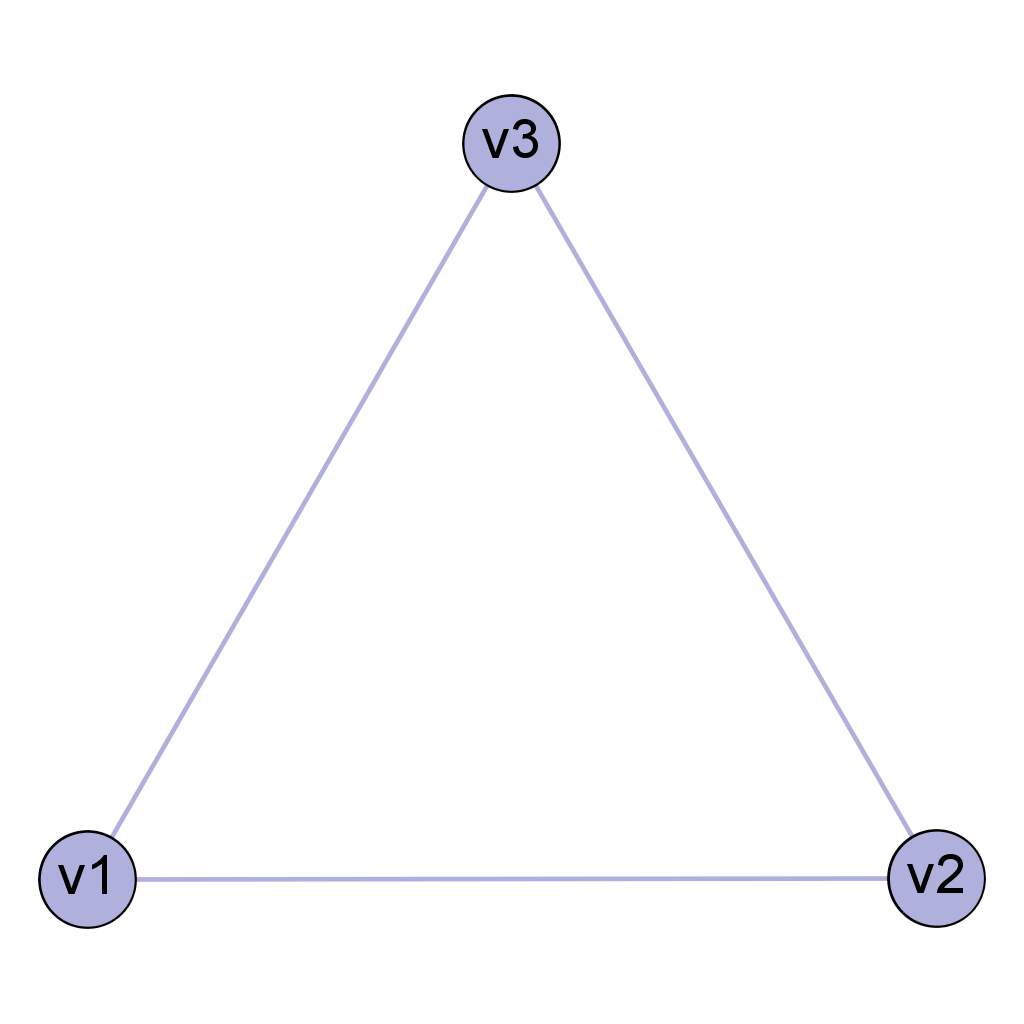
\includegraphics[width=.5\textwidth,height=.5\textheight,keepaspectratio]{images/clic_graph_3_node.png}
\end{figure}
\sethebrew

שאלה טביעית שנובעת כשגילנו שיש היא כמה פיתרונות יש למשחק מסוים.

\begin{theorem}
    מספר הפתרונות של משחק 
    שווה ל 
    $2^{k}$
    כאשר 
    $k$
    שווה לדרגת החופש של מטריצה
    $A$
    של פתרון הסטנדרתי
\end{theorem}

היות לכל משחק ניתן נהגיר מטריצת שכנויות של משחק שהגדרנו 
ב
\ref{def: neighbor matrix}
ופיתרונות של משחק וקטורים
$X$
של מערכת
$A X = \vec{1}$
כאשר 
$A$
מטריצת השכנויות.
ידוע שקיים פתרון למשחק ואם הוא משחק שמתחיל שכל נורות כבויות אז יש משפט 
\ref{thrm: clean game has solution}.
שמכויח זאת שקיים פיתרון.

היות ומניחים שיש כמה פיתרונות אפשר לתאר את כל פיתרונות כ
$x = x_n + x_0$
כאשר 
$x_n \in Nul(A)$ ,
$x_0$ 
פיתרון פרטי שידוע שקיים 
ו
$x$
כל פתרונות הכללים.

לכן מספר פתרונות כללים שווה למספר פיתרונות במרחב האפס.
ידוע שמספר פתרונות במרחב האפס שווה לדרגת החופש ולכן מספר הוקטורים שפורשים
את מרחב האפס שווה לדרגת החופש שנסמן ב
$k$.
כמות הווקטורים במרחב זה שווה לכל וקטורים שניתן ליצור בצירוף לינארי 
$x = a_1 x_1 + a_1 x_1 + a_2 x_2 + \cdots + a_k x_k$
כאשר הערכים של
$a_i \in Z_2$
לכן 
לכל מקדם יכול להיות
$2$
ערכים
לכן כל הקונבנציות האפשריות 
$2^k$
ששווה
לכמות הווקטורים 
במרחב האפס וכמות הפתרונות השונים של המשחק.

הבחנה נוספת ומעניינת שנרצה לציין היא בנושא חסם עליון לכמות הפיתרונות.
חסם עליון טרויאלי לכמות המקסמלית של פיתרונות היא 
$2^n$
פיתרונות כאשר
$n$
שווה למספר הלחצנים כלומר לא יכול להיות יותר פתרונות מאשר כמות הלחיצות השונות האפשריות במשחק.

\begin{comm}
    עבור משחק לוח מלבני
    בגודל 
    $m \times n$
    קיים לכל יותר 
    $2^k$
    כאשר 
    $k = \min{m,n}$
    פתרונות שונים
\end{comm}
הערה זאה נכונה לפי גישה פיתרון הספרדית
שהגדרנו
\ref{def: spanish way}
ניתן לתרגם את משחק ל
$k$
משוואות 
ש
$k$
יכול להיות מספר שורות או עמודות 
לכן ניקח את המספר הקטן יותר.

\section{פתרון מינימלי עבור לוחות מלבניים}



בפרק זה נציג פיתרון לבסוג מסוים של פתרונות שרצינו להציא סוג הפתרונות הללו
מביאים רמז וניראה שמקלים את משחק. הקלה שכזאת על משחק אולי 
יכולה לילצור הבונה חדשה ותת זווית חדשה למשחק כולו.

\begin{definition}
משחקים על לוח שקיים פיתרון שלחצנים 
שינו את מצב רק פעם אחת.
למשחקים כאלו נקיראה משחק מינמליים.
\end{definition}

באיור 
\ref{fig: min sol 2x3}
ניתן דוגמא לפתרון מינמלי 
בלוח 
$2 \times 3$.
כשלוחצים על לחצנים 
$2, 3$
על לוח כל נורות נדלקות ואף 
אחת מהם לא נכה באף שלב של לחיצה.

\begin{figure}[ht]
    \caption{פתרון מינמלי של משחק}
    \label{fig: min sol 2x3}
    \unsethebrew
    \centering
    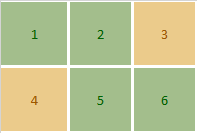
\includegraphics[width=.7\textwidth,height=.7\textheight,keepaspectratio]{images/min_sol_2x3.PNG}
\end{figure}
\sethebrew

השאלה שנפתור בפרק זה לאיזה לוחות קיים פתרון מימלי ופרק זה נראה 
מתקיימים על לוחות עם פתרון מינמלי.

\begin{definition}
    \label{def: dead zone}
    אזור מת זהו אוסף לחצנים בלוח
    שלחיצה עליהם 
    גורמת לחצן שכבר השתנה בעבר להשתנות שוב
\end{definition}

איזורים מתים על איור 
\ref{fig: min sol 2x3}
נראה שלאחר לחיצה על
לחצן
$2$
האזור מת שנוצר מלחיצה הינו
$\{0,1,2,4,5\}$

\begin{comm}
    אזור מת שנוצר מלחיצה 
    הוא כל הלחצנים במרחק לכל יותר 
    $2$
    משבצות מלחצן שנלחץ
    כאשר המרחק הוא מרחק מנהטן כלומר כל צדע למשבצת סמוכה למעלה למטה ימינה ושמאלה מגדילה את המרחק באחד
\end{comm}

\begin{figure}[ht]
    \caption{אזור מת שנוצר מלחצן באמצע הלוח}
    \label{fig: dead zone}
    \unsethebrew
    \centering
    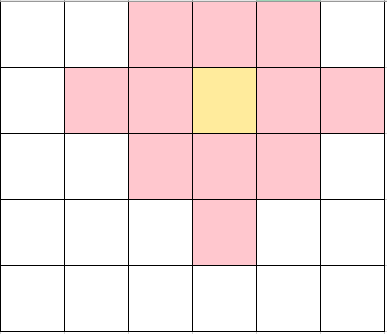
\includegraphics[width=.7\textwidth,height=.7\textheight,keepaspectratio]{images/dead_zone.PNG}
\end{figure}
\sethebrew

באיור 
\ref{fig: dead zone}
אפשר לראות שאם נלחץ על לחצן בצהוב האזור המת הי האזור באדום כולל 
הלחצן עצמו.
תכונה זה כלי מרכזי בהוכחה במשפט הבאה

\begin{theorem}
    \label{thrm: bigger then 7x7 board no minimal solution}
    במשחק על לוח 
    $m \times n$
    שמתקיים
    $\min(m,n) >= 7$
    למשחק אין פתרון מינמלי
\end{theorem}

נניח ויש לנו לוח דו מימדי שמתואר כך נקודת התחלה בכיוון למטה 
"קומת ראשונה"
והולך כלפי מעלה לאינסוף 
ואינסוף לצד ימין וצד שמאל.
נקרה לכל עליה בגובה
קומה ונמספר אותם מאחת לאינסוף לכן קראנו לקומה נמוכה ביותר קומה ראשונה
נרצה לתא על לוח כזה את כל מקרים האפשרים ואיזורים האסורים שנמצאים על הלוח.
נרצה למצוא פיתרון מינמלי ללוח
וגישה לחיפוש הפתרון תהיה
להדליק שורה אחר שורה במלואה,
היות ושורת אינסופיות נציעה אסטרטגיה להדלקת השורה וניראה את הקשיים שנפגוש.
אם נירצה להדליק 
את כל קומה ראשנה רק על ידי לחצות 
בשורה ראשונה נקבל את הדפוס 
שאם לחצתי על לחצן מסוים חייב אני ללחוץ על לחצן
$3$
מימינו
כמו שמתואר באיור
\ref{fig: fill first stage only pressing first stage}
שמתאר לחצנים בירוק כלחצנים שנלחצו 
צהוב לחצנים שנלדקו ובאדום אזורים מתים שלא נדלקו.
באיור מוצג רק שתי לחצות עוקבות של אסטרטגיה אבל כך נדליק את השורה הראשונה.

נשים לב באיור 
\ref{fig: fill first stage only pressing first stage}
על שני אזורים המתים הצמודים שלא נדלקו שצמודים אחד לשני כדי להדליק את שינהם
לא נוכל לעשות זאת ללא כיבוי לחצן שכבר נדלק.
זאת אומר שאסטרטגיה שכזאת
נפסלת עבור מילוי משחק שקומה שלו גדולה מ
$1$.

\begin{figure}[ht]
    \caption{מילוי קומה ראשונה על ידי לחיצות רק בקומה ראשונה}
    \label{fig: fill first stage only pressing first stage}
    \unsethebrew
    \centering
    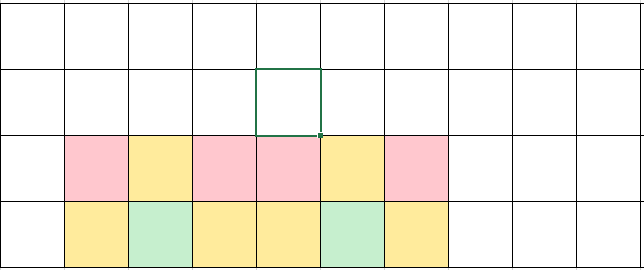
\includegraphics[width=.7\textwidth,height=.7\textheight,keepaspectratio]{images/first_stage_fill_only_first_stage_click.PNG}
\end{figure}
\sethebrew

אסטרטגיה אחרת ויחידה למילוי קומה ראשונה הינה להדליק 
פעם לחצן בקומה ראשנה 
ופעם לחצן בקומה שניה צמודים כפי שנוכל.
היות ואפשר רק בעזרת לחיצות בשני שורות עלו ולא רוצים שני לחיצות עוקבות
בקומה ראשונה זה היא האסטרטגיה האלטרנטיבית היחידה.

\begin{figure}[ht]
    \caption{מילוי קומה ראשונה}
    \label{fig: fill first stage second attempt}
    \unsethebrew
    \centering
    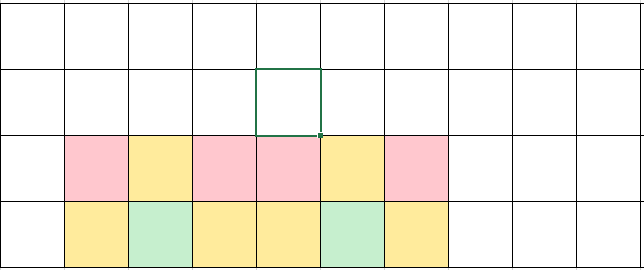
\includegraphics[width=.7\textwidth,height=.7\textheight,keepaspectratio]{images/first_stage_fill_only_first_stage_click.PNG}
\end{figure}
\sethebrew

באיור 
\ref{fig: fill first stage second attempt}
אפשר לראות הדגמה קטנה של אסטרטגיה שכזה.

נרצה להראות אסטרטגיה שכזה מובילה לאזורים מתים שלא ניתן למלאות 
כל עוד רוצים שהפתרון היה מינימלי.
אם נסתכל באיור 
\ref{fig: fill first stage second attempt fails}
ניראה שאזורים המתים ששלשת
המשבצות הרצופות באדום לא ניתן היה למלאה אותם לכן צירוף כזה אין חוקי
כלומר הראינו שלמשחק על בצורה שהגדרנו.

\begin{figure}[ht]
    \caption{מילוי קומה ראשונה}
    \label{fig: fill first stage second attempt fails}
    \unsethebrew
    \centering
    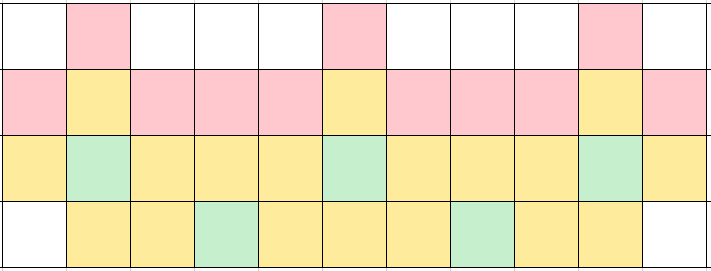
\includegraphics[width=.7\textwidth,height=.7\textheight,keepaspectratio]{images/first_stage_fill_only_first_stage_click_fail.PNG}
\end{figure}
\sethebrew

בשלב זה נירצה להקטין את הרוחב ואורך כך שאם קיים 
משחק אופטמלי בלוח המוקטן אסטרטגיות המילוי קומה קומה היחידות 
שהיו חוקיות הן עלו שהצגנו.
נדע שהקטנה לא היו לה פיתרונות אופטמלים אם היו משבצות סמוכות באזורים מתים.

נחזור ונסתכל על איור 
\ref{fig: fill first stage only pressing first stage}
נשים לב שלכל לוח שמפסר המשבצות לרוחב גדול או שווה 
מ
$6$
שיטת המילוי שכזה תהיה לא חוקית כי היו 
$2$
משבצות סמוכות שבאיזורים לא חוקיים.
ובאיור 
\ref{fig: fill first stage second attempt fails}
ניראה
שלרוחב גדול או שווה 
מ
$5$
היות ובניה
של קומה ראשונה מסמכת על זה שיש 
$7$
משבצות ניקח ליתר ביטחון 
$7$
משבצות ולאחריהם  לרוחב ולכן באסטרטגיה זאה לא היה פיתרון מינמלי.

קיבלנו שאפשר להקטין את הלוח לרוחב של
$7$
משבצות 
ועדיין לא היה פתרון  מינמלי. 

את אותם טענות אובניה אפשר היה לבנות לא רק להגביל את רוחב ל
$7$
משבצות עלה גם לגובה.
לכן לסיכום קיבלנו 
במשחק על לוח 
שאורך או רוחב גדולים או שווים מ
$7$
אז
למשחק אין פתרון מינמלי
והוכחנו את הטענה.


\subsection{הלוח הגדול ביותר בעל פיתרון מינמלי}

טענה 
\ref{thrm: bigger then 7x7 board no minimal solution} 
מקבילה מאד את המשחקים שיש להם פתרון מינמאלי ובשיטת הפתרון שהצגנו
אחד המסקנות המתקבלות שאם יש שלוש קומות או יותר מתחילה
להיות בעיתות בגישת מילוי השורות.
אפשר להבחין בתופעה זה היות וקיים פתרון למשחק 
$2 \times m$
כאשר 
$m$
הוא איזוגי
האסטרטגיה השנייה מאפשרת מילוי קומות ולקבל פיתרון מינמלי
נדגים זאת על באיור 
\ref{fig: 2x9 have min sol}

\begin{figure}[ht]
    \caption{פתרון ללוח 
    $2 \times 9$}
    \label{fig: 2x9 have min sol}
    \unsethebrew
    \centering
    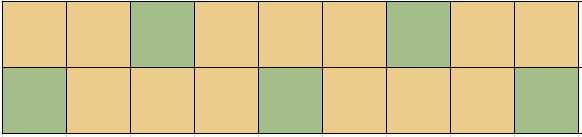
\includegraphics[width=.7\textwidth,height=.7\textheight,keepaspectratio]{images/2xm_sol.PNG}
\end{figure}
\sethebrew

לאחר שהבנו שלוחות בגודל 
$2 \times m$
כאשר 
$m$
איזוגי 
קיים פיתרון מינמלי נשאל מהו הלוח 
הגדול ביותר
בעל פיתרון מינמלי כאשר 
הלוח אורך ורוחב גדולים מ
$2$.

לפי טענה 
\ref{thrm: bigger then 7x7 board no minimal solution} 
אין טעם לבדוק לוחות שעמודות ושורות גדולים מ
$7$
ומבניית ההוכחה 
אמרנו שאם 
הגדול של עמודות או שורות לא קטן
מ
$3$
לכן גם אין טעם לבדוק 
שורות ועמודות גדולים מ
$7$
כלומר נותר לבדוק לוחות שמימד שלהם 
$m \times n$
שייכים לקבוצה
$\{ (m,n) : 2 < m,n <7 \}$.

אפשר לנסות ולחפש פיתרון ידנית
או לעבור על כל הפיתרונות של משחק רגיל ולבדוק עם יש מבינהם פיתרון 
מינמלי.
נציאה דרך אחרת לחפש פיתרון 
והיא בעזרת לשתמש באותה מטריצה כפי שהגדרנו רק להגדיר 
את שהיא על חוג 
$\mathbb{Z}$.
בעזרת שימוש בחוג 
$\mathbb{Z}$
מאלצים שפתרון המתקבל 
ידליק כל נורות אך ורק פעם אחת,
זאת מתקיים בעקבות 
משוואות האילצים שהגדרנו ב
\ref{ def: depndeciy equation}
שמאלצות את הסכום להיות שווה לאחד
,
אם ניסתכל על נוסחה של משוואת האילצים הכללים 
נוסחה
\ref{eq: depndeciy equation}
היות וחבור על השלמים לכן 
מאולצים במשוואה זה שהיה לחצן בודד לחוץ 
לכן פיתרון מערכת המשוואות מתאר פיתרון 
מינמלי של משחק.
התיאוריה שפיתחנו באלגברה לינארית היתה תקפה לשדות 
אבל כלי תכנות שהשתמשנו
בעבודה זה יודע לפתור גם על חוג של השלמים 
והסמכנו על הכלי כדי לבדוק את המקרים
שמימדים שייכם לקבוצה 
$\{ (m,n) : 2 < m,n <7 \}$
וקיבלנו שהלוח
היחיד בקוצת המימדים העלו שיש לו פיתרון מינמלי 
הוא
לוח 
$4 \times 4$
ופיתרון מתואר באיור 
\ref{fig:4x4_have_min_sol}

\begin{figure}[ht]
    \caption{פתרון ללוח 
    $4 \times 4$}
    \label{fig:4x4_have_min_sol}
    \unsethebrew
    \centering
    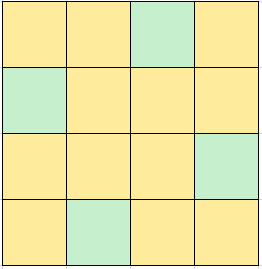
\includegraphics[width=.7\textwidth,height=.7\textheight,keepaspectratio]{images/4x4_min_sol.PNG}
\end{figure}
\sethebrew

\newpage

\section{נספחים}
מימוש של הפרויקט בוצע על ידי 
שפת תוכנה 
\L{Python}
עם הכלי 
\L{Sage}.

\unsethebrew
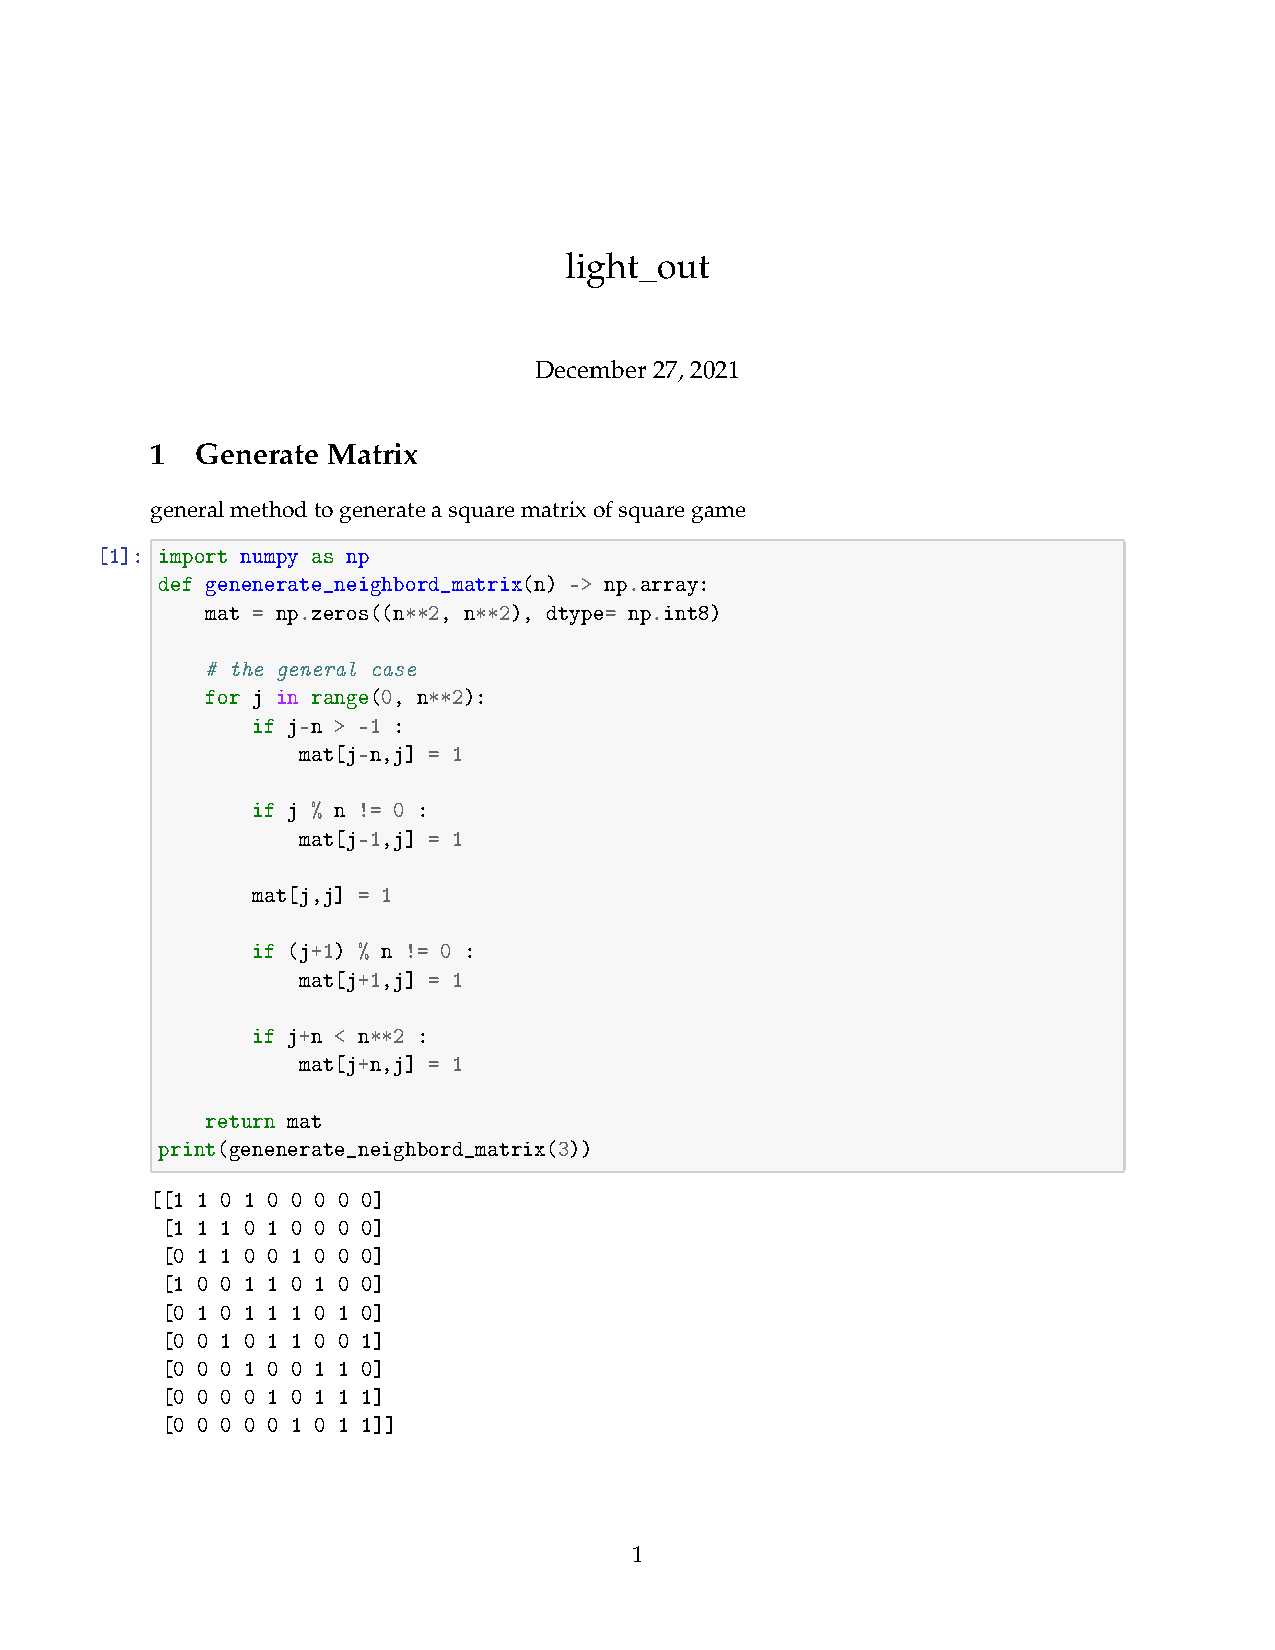
\includepdf[pages=-]{light_out_jupyter.pdf}
\sethebrew
%----------------------------------------------------------------------------------------
%   רשימת מקורות
%----------------------------------------------------------------------------------------
\newpage
\begin{thebibliography}{99}
\unsethebrew
\bibitem{B1} ALL LIGHTS AND LIGHTS OUT
An investigation among lights and shadows by
SUMA magazine’s article by Rafael Losada
Translated from Spanish by Ángeles Vallejo

\bibitem{B2} Lecture 24: Light out Puzzle , SFU faculty of scienc department of mathematics
\bibitem{B3} algebra book TODO: fill it
\end{thebibliography}

\end{document} 
